\documentclass[12pt]{article}
\usepackage{paper,math}
\usepackage[margin=1in]{geometry}
\addbibresource{references.bib}
\usepackage[linesnumbered,ruled,vlined]{algorithm2e}
\usepackage{amsmath}  % If you're using math symbols
\usepackage{amsfonts} % O

\title{Gene Set Enrichment Analysis \\-\\ Genomorientierte Bioinfromatik}
\author{Malte Weyrich}
\date{\today}
% Conditionally display thoughts (hide by switching to `\boolfalse`)
% \booltrue{INCLUDECOMMENTS}
\newcommand{\malte}[1]{\coauthorComment[Malte]{#1}}

\begin{document}

% Title Page -------------------------------------------------------------------
\maketitle
\begin{abstract}


\end{abstract}

\newpage


% Paper ------------------------------------------------------------------------

% ------------------------------------------------------------------------------
\section{Introduction}\label{sec:Introduction}
Due to the vast amount of different genes and gene products, a vocabulary for describing
groups of genes and their logical relationships, called \textit{\textbf{Gene Ontology
(GO)}}, was invented by the \textit{\textbf{Gene Ontology Consortium (GOC)}} (\cite{Ashburner2000}).
In \textit{Gene Ontology}, genes are sorted into different \textit{gene sets} (referred
to as \textit{GO Terms}), with each gene set having its own ID.
These gene sets are annotated with a function and a process,
in which the genes of the set are involved in. A gene set can be a component of several
another gene sets through an \textit{is\_a relationship}, which leads to a hierarchical,
tree-like structure. In this case the structure is a \textit{\textbf{Directed Acyclic
Graph (DAG)}}. The biological functions and processes are sorted into three main categories:
\textit{Biological Process (BP)}, \textit{Molecular Function (MF)} and \textit{Cellular
Component (CC)}, each forming its own \textit{DAG}. The root of each \textit{DAG}
comprises all genes of the \textit{DAG} and is labeled with the one of the \textit{GO
Terms}. The amount of genes per gene set is decreasing the further its location is
relative to the root. Same goes for the annotations of gene sets, which get more exact
and detailed the further they are away from the root. 

In bioinformatics, this vocabulary is crucial for determining the effects of differentially
expressed genes in RNA-seq and other experiments. Knowing which genes are significantly
up or down regulated is not sufficient enough for understanding the biological processes
that are affected by the changes in gene expression. This is where \textit{\textbf{Gene
Set Enrichment Analysis (GSEA)}} and \textit{\textbf{Gene Over-representation Analysis
(ORA)}} come into play. Although these two methods differ in their methodology, the
main goal is to determine, whether certain gene sets are statistically enriched or
not, providing insights into affected biological pathways.

The analysis conducted in this report tries to compare the results of both methods
for a given list of differentially expressed genes and standard of truth gene sets.
Additionally, our results are compared to two already existing tools for \textit{ORA}, called
\textit{\textbf{gProfiler}} (\cite{gprofiler}) and \textit{\textbf{fgsea}} (\cite{fgsea})
for \textit{GSEA}.

\section{Materials \& Methods}
\subsection{Enrichment Methods}\label{sec:Enrichment-Methods}
\subsubsection{Gene Set Over-representation Analysis}\label{sec:Gene-Set-Over-representation-Analysis}

\subsubsection{Gene Set Enrichment Analysis}\label{sec:Gene-Set-Enrichment-Analysis}

\newpage
\subsection{Java Programm}\label{sec:Java-Programm}
The provided \textit{JAR} has the following input specification:
\begin{verbatim*}
java -jar go_enrichment.jar
  -obo                   Path to obo file.
  -root                  One of three Ontology Terms:
                         ["molecular_function",
                         "biological_process",
                         "cellular_component"].
  -mapping               Path to mapping file (SYMBOL -> GO_ID).
  -mappingtype           Format of the mapping-File (go|ensembl). 
                         Has to agree with "-mapping" option.
  [-overlapout]          Information about DAG  entries  with shared mapped
                         genes is written into this file.
  -enrich                Path to enrichment analysis file.
  -o                     Path to output file.
  -minsize               Min amount of genes per GO entry.
  -maxsize               Max amount of genes per GO entry.
\end{verbatim*}

The specific file formats are described in \textit{Assignment 5}.
\newpage
\subsubsection{Logic}\label{sec:Logic}
\textbf{(A) Parsing Input Files:}

The provided \textit{JAR} reads in the necessary input files and stores for later use.
Parsing the \textit{obo} file is the first step, since it contains the structure
of the \texttt{DAG}, which itself is an object. The parser only considers entries which map
the parameter \textit{"-root"} and ignores entries which are marked as obsolete.
It stores entries in a \texttt{HashMap<String, GOEntry> nodeMap} to keep 
track of already seen gene sets. For each entry, we check if
its GO id is contained in our \texttt{nodeMap}. If not, we simply append
a new \texttt{GOEntry} object to \texttt{nodeMap} and add its parents 
to the newly created object. Otherwise, we take the already existing \texttt{GOEntry} 
object inside the \texttt{nodeMap} and update its parents. 
Of course we also have to look up parent GO ids inside \texttt{nodeMap}
before creating a new \texttt{GOEntry} object. This way we can ensure that 
the \texttt{DAG} is correctly built up. The \texttt{root} of the \texttt{DAG} is
the obo entry which has the same name as the parameter \textit{"-root"}.

Based on the provided \textit{"-mappingtype"}, the \textit{JAR} has two different 
methods for parsing the file specified in \textit{"-mapping"}. 
This part populates the created \texttt{DAG} object with the gene symbols.
The symbols are stored as a \texttt{HashSet<String> geneSymbols} in each \texttt{GOEntry} object.
Lastly, the \textit{JAR} reads in the enrichment analysis file and stores the results
in a \texttt{HashMap<String, Gene> enrichedGeneMap}. The first lines of our enrichment file
also contains standard of truth (SoT) GO ids, which are gene sets that are known to be
enriched for the given list of differentially expressed genes. These SoT GO ids are 
used to mark the corresponding \texttt{GOEntry} objects in the \texttt{DAG} and are
additionally stored in a \texttt{HashSet<GOEntry> trueGoEntries}. We will use this
for later comparisons.\\
\hspace{1mm}
\hspace{1mm}
\textbf{(B) Preparing DAG for Enrichment Analysis:}

At this point of the program, we have a fully constructed \texttt{DAG} object.
As described in \ref{sec:Introduction}, a parent \texttt{GOEntry} object
inherits all genes from its children.
Calling the method \texttt{inheritGeneSymbols()} on the \texttt{root} of the \texttt{DAG}
leads to an recursive update of the gene symbols in each \texttt{GOEntry} object
from the bottom to the top of the \texttt{DAG}. After this step, the \texttt{root}
contains all gene symbols of the \texttt{DAG}. The same logic is used to 
create a \texttt{HashSet<String> reachableGOIDs} in each \texttt{GOEntry} object,
which will be useful for later calculations. The result file should also contain
a field called \textit{"shortest\_path\_to\_a\_true"}. This field is supposed to
describe the shortest path from a \texttt{GOEntry} $A$ to the closest true
\texttt{GOEntry} $B$. 
These paths can be pre-computed, avoiding expensive breadth-first searches which
might compute the same path multiple times.
For this purpose, each \texttt{GOEntry} object has a 
field \texttt{HashMap<GOEntry, LinkerClass> HighwayMap} which stores the
true \texttt{GOEntries} \textbf{as keys} and a \texttt{LinkerClass} object as value.
The \texttt{LinkerClass} object contains the \texttt{GOEntry} object
\textbf{which has to be traversed} to reach the true \texttt{GOEntry} and
a value $k$ which describes the remaining distance to the true \texttt{GOEntry}.

\begin{figure}[htpb]
    \centering
    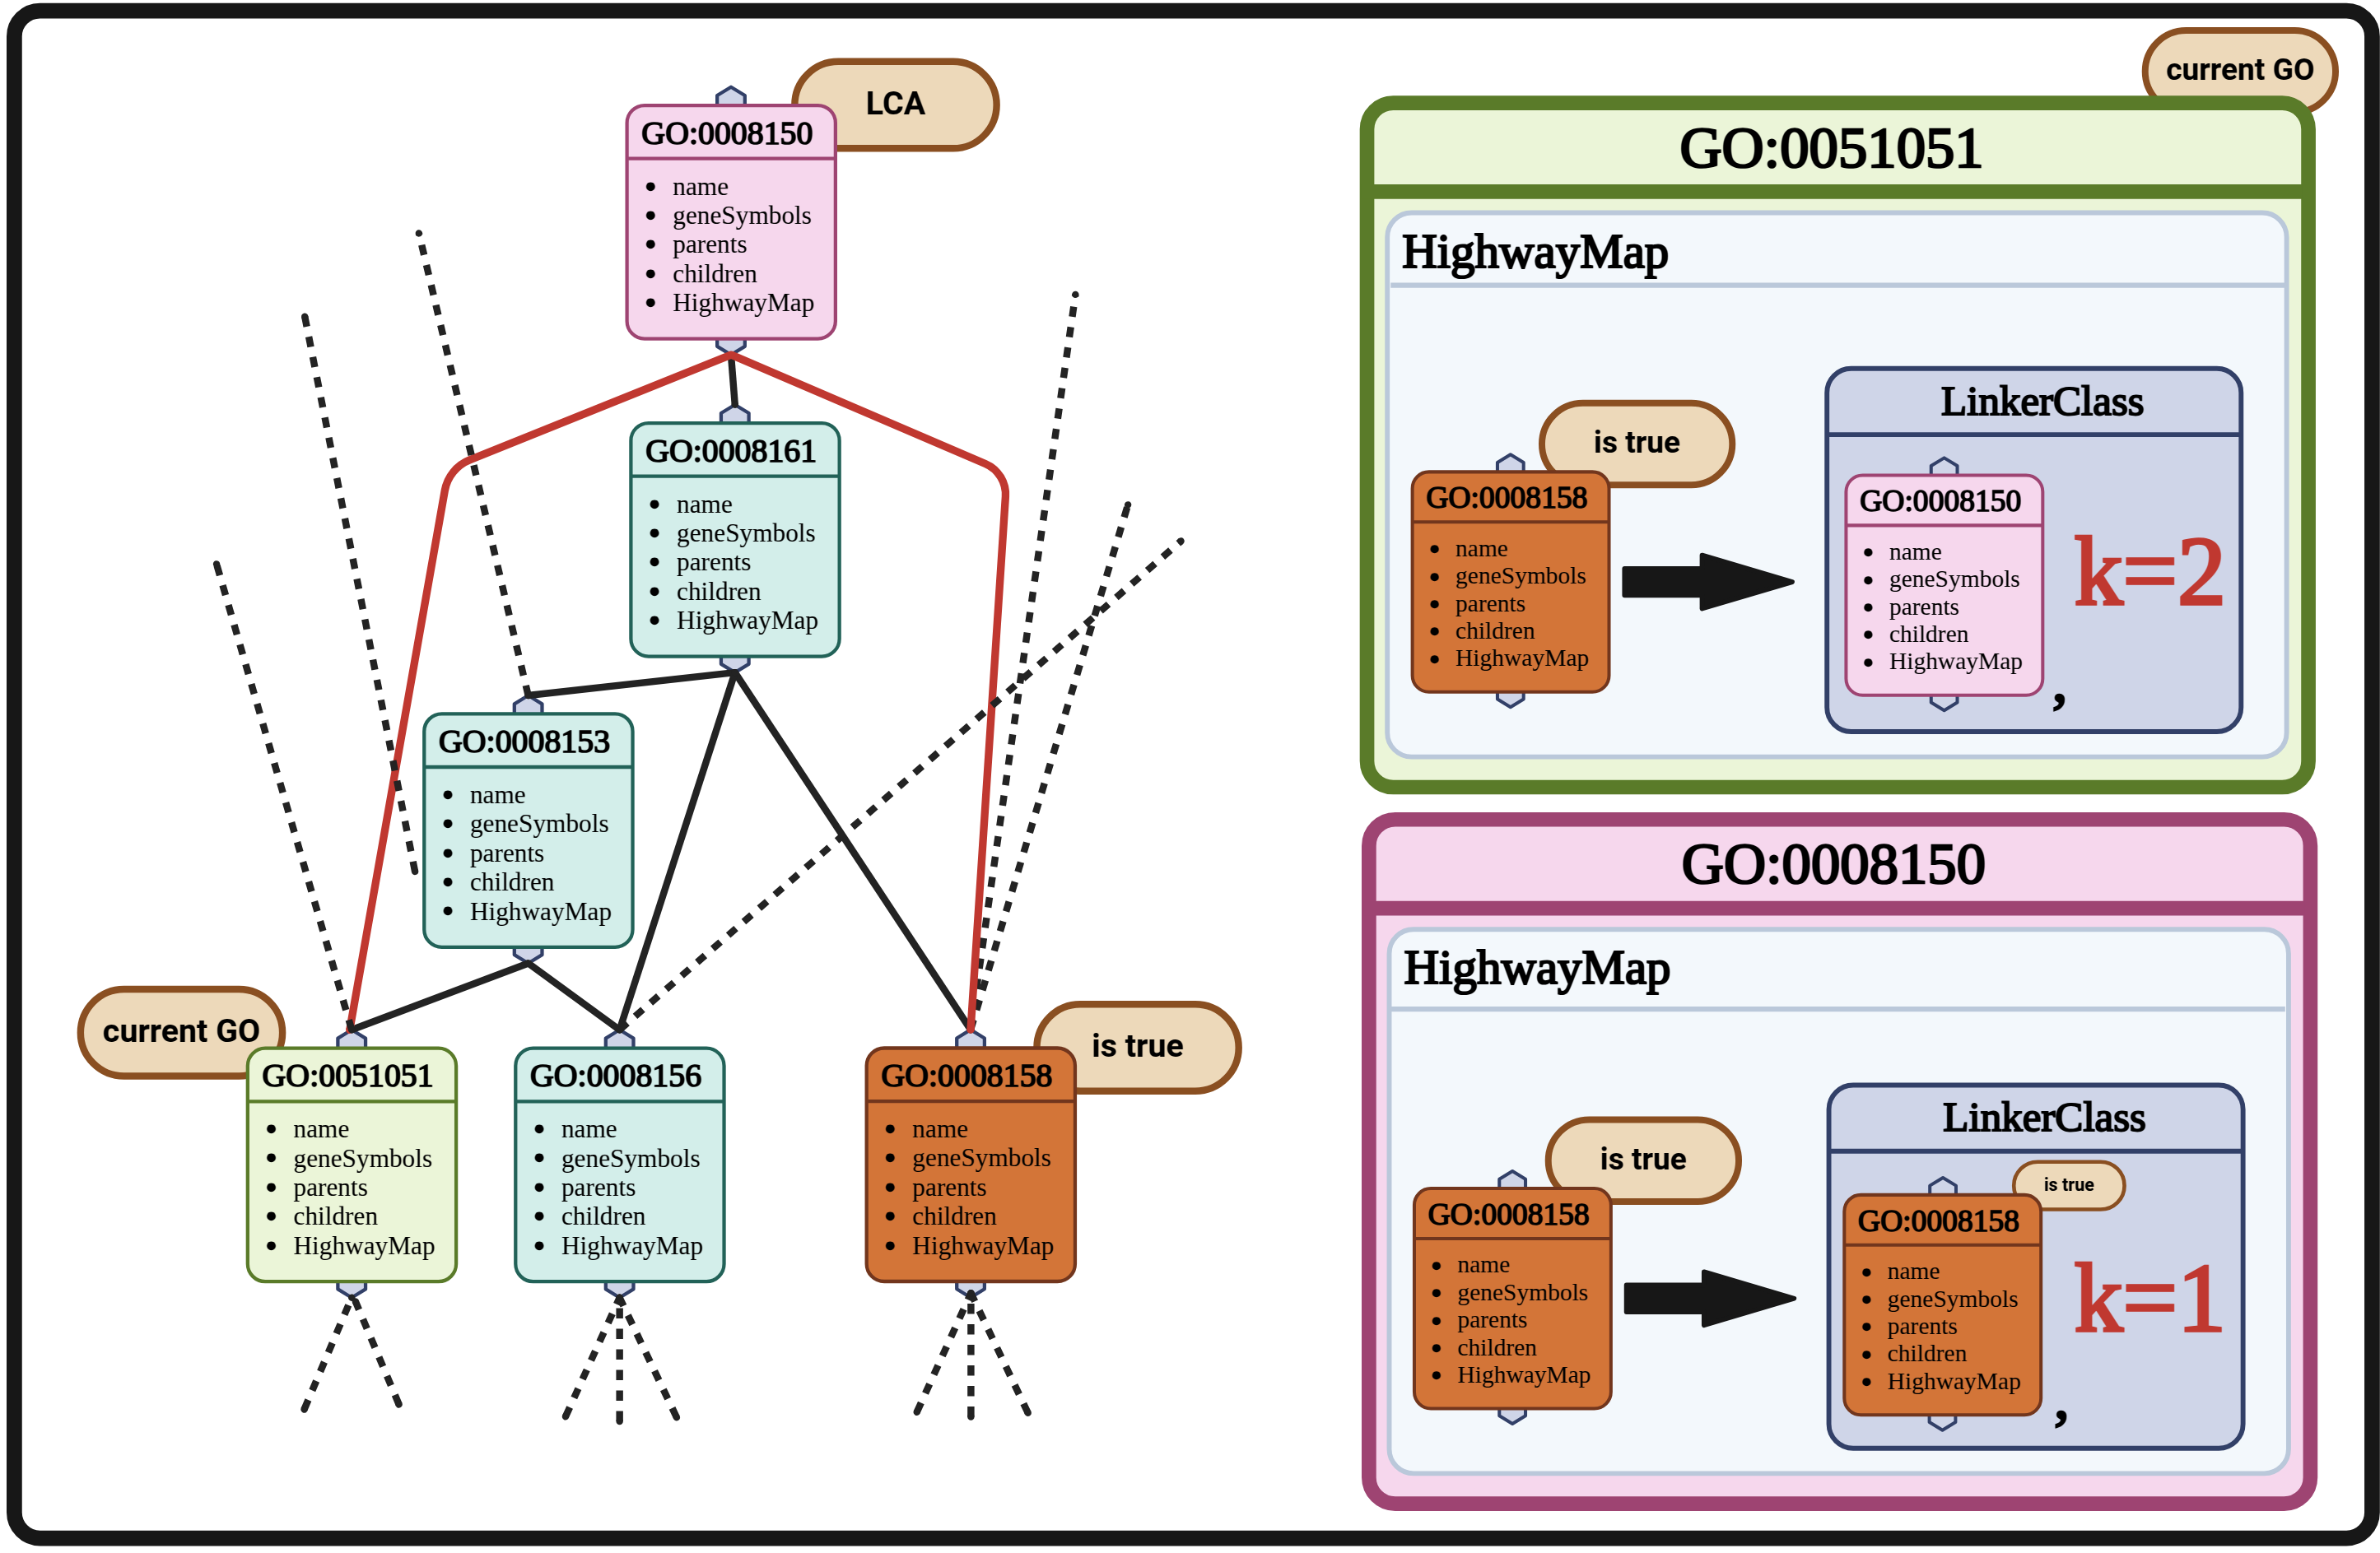
\includegraphics[width=0.99\textwidth]{./figures/Highway.png}
    \caption{A simple example of how the \texttt{HighwayMap} uses the true \texttt{GOEntries} as key and stores a \texttt{LinkerClass} object as value,
    serving as a highway to the true \texttt{GOEntry}.}
    \label{fig:-figures-Highway-png}
\end{figure}


We start populating the \texttt{HighwayMap} with the true \texttt{GOEntries}
by fist calling the method \texttt{signalShortestPathUp(0, GOEntry trueGO)} (Algorithm \ref{alg:signalShortestPathUp}) on each true \texttt{GOEntry}.
This method is called recursively on each parent of the true \texttt{GOEntry} and
propagates the shortest path to the true \texttt{GOEntry} upwards in the \texttt{DAG}.
This alone is not sufficient, since we also have to propagate the shortest path
downwards in the \texttt{DAG}. 
For this purpose, we call the method \texttt{propagateShortestPaths(trueGo)} (Algorithm \ref{alg:propagateShortestPaths}) on the \texttt{\textbf{root}} 
of the \texttt{DAG}.
While the method \texttt{propagateShortestPaths()} ensures that the shortest paths propagate 
down from the \texttt{root}, it doesn't explicitly finalize the correct shortest 
paths for every node. This is done by calling the method \texttt{signalShortestPathDown(0, trueGo)} (Algorithm \ref{alg:signalShortestPathDown}) on all true \texttt{GOEntries}.
It makes sure that once the shortest paths are propagated down from the \texttt{root}, 
every node (especially those closer to \texttt{trueGo}) has the correct, 
finalized shortest path to the trueGo.

\begin{algorithm}[!htbp]
\caption{signalShortestPathUp(k, trueGo)}\label{alg:signalShortestPathUp}
\KwIn{$k$, trueGo}
\KwOut{Updated shortest path values for all parents}
\ForEach{parent in parents}{
    \If{parent.highwayMap does not contain trueGo}{
        link = new LinkerClass(this, k + 1) \;
        parent.highwayMap.put(trueGo, link) \;
    }
    \ElseIf{parent.highwayMap.get(trueGo).getK() > k + 1}{
        parent.highwayMap.get(trueGo).setGo(this) \;
        parent.highwayMap.get(trueGo).setK(k + 1) \;
    }
    parent.signalShortestPathUp(k + 1, trueGo) \;
}
\end{algorithm}


\begin{algorithm}[!htbp]
\caption{propagateShortestPaths(trueGo)}\label{alg:propagateShortestPaths}
\KwIn{trueGo}
\KwOut{Updated shortest path values for all descendants}
currentPath $\gets$ highwayMap.get(trueGo) \;
\If{currentPath is not null}{
    nextNode $\gets$ currentPath.getGo() \;
    \If{nextNode.highwayMap contains trueGo}{
        pathThroughLinker $\gets$ nextNode.highwayMap.get(trueGo).getK() + 1 \;
        \If{pathThroughLinker < currentPath.getK()}{
            currentPath.setK(pathThroughLinker) \;
        }
    }
}
currentK $\gets$ currentPath is not null ? currentPath.getK() : \texttt{Integer.MAX\_VALUE} \;
\ForEach{child in children}{
    childPath $\gets$ child.highwayMap.get(trueGo) \;
    childK $\gets$ childPath is not null ? childPath.getK() : \texttt{Integer.MAX\_VALUE} \;
    \If{currentK is not \texttt{Integer.MAX\_VALUE} and currentK + 1 < childK}{
        \If{childPath is null}{
            childPath $\gets$ new LinkerClass(this, currentK + 1) \;
            child.highwayMap.put(trueGo, childPath) \;
        }
        \Else{
            childPath.setGo(this) \;
            childPath.setK(currentK + 1) \;
        }
    }
    child.propagateShortestPaths(trueGo) \;
}
\end{algorithm}


\begin{algorithm}[!htbp]
\caption{signalShortestPathDown(k, trueGo)}\label{alg:signalShortestPathDown}
\KwIn{$k$, trueGo}
\KwOut{Updated shortest path values for all descendants}
k $\gets$ k + 1 \;
\ForEach{child in children}{
    \If{child.highwayMap does not contain trueGo}{
        link $\gets$ new LinkerClass(this, k) \;
        child.highwayMap.put(trueGo, link) \;
    }
    \ElseIf{child.highwayMap.get(trueGo).getK() > k}{
        child.highwayMap.get(trueGo).setGo(this) \;
        child.highwayMap.get(trueGo).setK(k) \;
    }
    child.signalShortestPathDown(k, trueGo) \;
}
\end{algorithm}

\newpage
\hspace{1mm}\\
\textbf{(C) Enrichment Analysis:}

The actual enrichment analysis is conducted in the method \texttt{analyzeParallel()} of the
class \texttt{EnrichmentAnalysis}. This method iterates over all \texttt{GOEntry} objects
and checks, whether their amount of genes is within the specified range of \textit{"-minsize"}
and \textit{"-maxsize"}. 
An object called \texttt{AnalysisEntry} is created for each \texttt{GOEntry} object which
fulfills the requirements.
It then calculates the overlap of the gene symbols of the current \texttt{GOEntry} with 
the gene symbols of the differentially expressed genes and stores the result 
in the \textit{"size"} field of the \texttt{AnalysisEntry} object ($\equiv n$).
The attribute \textit{"noverlap"} is the amount of significantly differentially expressed genes
which also occur in the current \texttt{GOEntry} ($\equiv k$). 
The universe size is the intersection of all gene symbols of the differentially expressed genes
and all gene symbols of the \texttt{DAG} ($\equiv N$). Lastly, $K$ is the amount of significantly
differentially expressed genes intersected with all gene symbols of the \texttt{DAG}.
For the komogorov-smirnov test we define the following values:
\begin{itemize}
    \item[\textbf{I.}] \textit{In-Set Distribution}: Genes present in the current \textit{GOEntry} and differentially expressed genes.
    \item[\textbf{II.}] \textit{Background Distribution}: Genes not in the \textit{In-Set} but part of the background gene pool.
\end{itemize}
For both of these distributions, we store the \textit{logFoldChange} values of the differentially
expressed genes into two arrays.
With these values, the statistical tests described in \ref{sec:Enrichment-Methods} are 
conducted to determine the significance of the enrichment of the current \texttt{GOEntry}. 
As a result we obtain the following values and store them in the \texttt{AnalysisEntry} object:
\begin{itemize}
    \item \textit{hgPval}: Hypergeometric p-value.
    \item \textit{fejPval}: Jackknife Fisher's Exact Test p-value.
    \item \textit{ksPval}: Kolmogorov-Smirnov p-value.
    \item \textit{ksStat}: Kolmogorov-Smirnov statistic ($\equiv$ \textit{Enrichment Score}).
\end{itemize}
\hspace{1mm}\\
Now we calculate the shortest path to the closest true \texttt{GOEntry} for each \texttt{AnalysisEntry}
by utilizing the pre-computed \texttt{HighwayMap} of the current \texttt{GOEntry}.
We simply choose the \texttt{GOEntry} object which points to the \texttt{LinkerClass}
with the smallest $k$ value in the \texttt{HighwayMap} as our \texttt{target GOEntry}. 
For each visited \texttt{GOEntry} object on the path, we check
if the \texttt{HighwayMap} still contains the \texttt{target GOEntry} as key.
If so, we follow its \texttt{LinkerClass} object until we reach the \texttt{target}.
We know when we hit the \textit{least common ancestor (LCA)} of the current \texttt{GOEntry}
and the closest true \texttt{GOEntry},
by checking if the \texttt{reachableGOIDs} object contains our \texttt{target GOEntry}
for each visited \texttt{GOEntry} object on the current path.

After all \texttt{AnalysisEntry} objects have been processed, 
all p-values are corrected for multiple testing using the \textit{Benjamini-Hochberg}
method. The corrected p-values are stored in the \texttt{AnalysisEntry} objects
and each object is written to the output file.
The above procedure is conducted in parallel in order to speed up the process.
\hspace{1mm}\\
\textbf{(D) GO Features:}

The optional parameter \textit{"-overlapout"} specifies an additional 
output file which stores further features of the underlying \texttt{DAG}.
For this, each unique pair of \texttt{GOEntries} $(A,B)$ fulfilling the
\textit{"-minsize"} and \textit{"-maxsize"} parameter are 
intersected by their \textit{gene symbols}. If there is an overlap,
we calculate the shortest path in between $A$ and $B$.
In this case we use a \textit{Breadth-First Search} algorithm
to explore all ancestors of $A$ and $B$ and return the shortest path.
Additionally we write a \texttt{boolean} value into the output file
which indicates whether $A$ can be directly reached from $B$ or vice versa.
Lastly, we store the max percentage of shared genes between $A$ and $B$:
\[
    \textit{max percentage} = \frac{|A \cap B|}{\textit{max}\left\{|A|, |B|\right\}} \times 100
.\]


\subsubsection{Runtime}\label{sec:Runtime}
\section{Results}
\subsection{DAG Properties}\label{sec:DAG-Properties}

\begin{table}[htpb]
    \centering
    \caption{DAG Properties summary. The table shows the number of genes, gene sets, leafs, the length of the shortest $S$ and longest $L$ path to the \texttt{root} in the DAG.}
    \label{tab:dag_properties}
\begin{tabular}{|c|c|c|c|c|c|} \hline
     \textbf{Mapping Type} & \#Genes & \#\texttt{GOEntries} & \#Leafs & $S$ & $L$ \\ \hline
     \textbf{GO} & 17026 & 29385 & 14991 & GO:0031629 $\to$ 2 & GO:1905741 $\to$ 17 \\ \hline
 \textbf{ENSEMBL} & 15496 & 29385 & 14991 & GO:0031629 $\to$ 2 & GO:1905741 $\to$ 17 \\ \hline
\end{tabular}
\end{table}

Table \ref{tab:dag_properties} shows the properties of the \texttt{DAG} for both mapping
types. The \texttt{DAG} itsself contains 29385 gene sets, with 14991 leafs. The shortest
path to the \texttt{root} is 2 edges long, while the longest path is 17 edges long.
These properties are the same for both mapping types, since the \texttt{DAG} structure is the
same for both mapping types. The only difference is the gene symbols which are stored in the \texttt{GOEntries} (15496 vs. 17026).
Figure \ref{fig:-plots-goSizes-png} additionally shows the distribution of gene set sizes in the \texttt{DAG} for both mapping types,
as well as the difference in gene set sizes between parent and child nodes.
It seems that the difference in gene set size per traversed edge is slightly more pronounced for the \texttt{GO} mapping type compared to the \texttt{ENSEMBL} mapping type,
while the overall distribution of gene set sizes is similar for both mapping types.


\begin{figure}[!htbp]
    \centering
    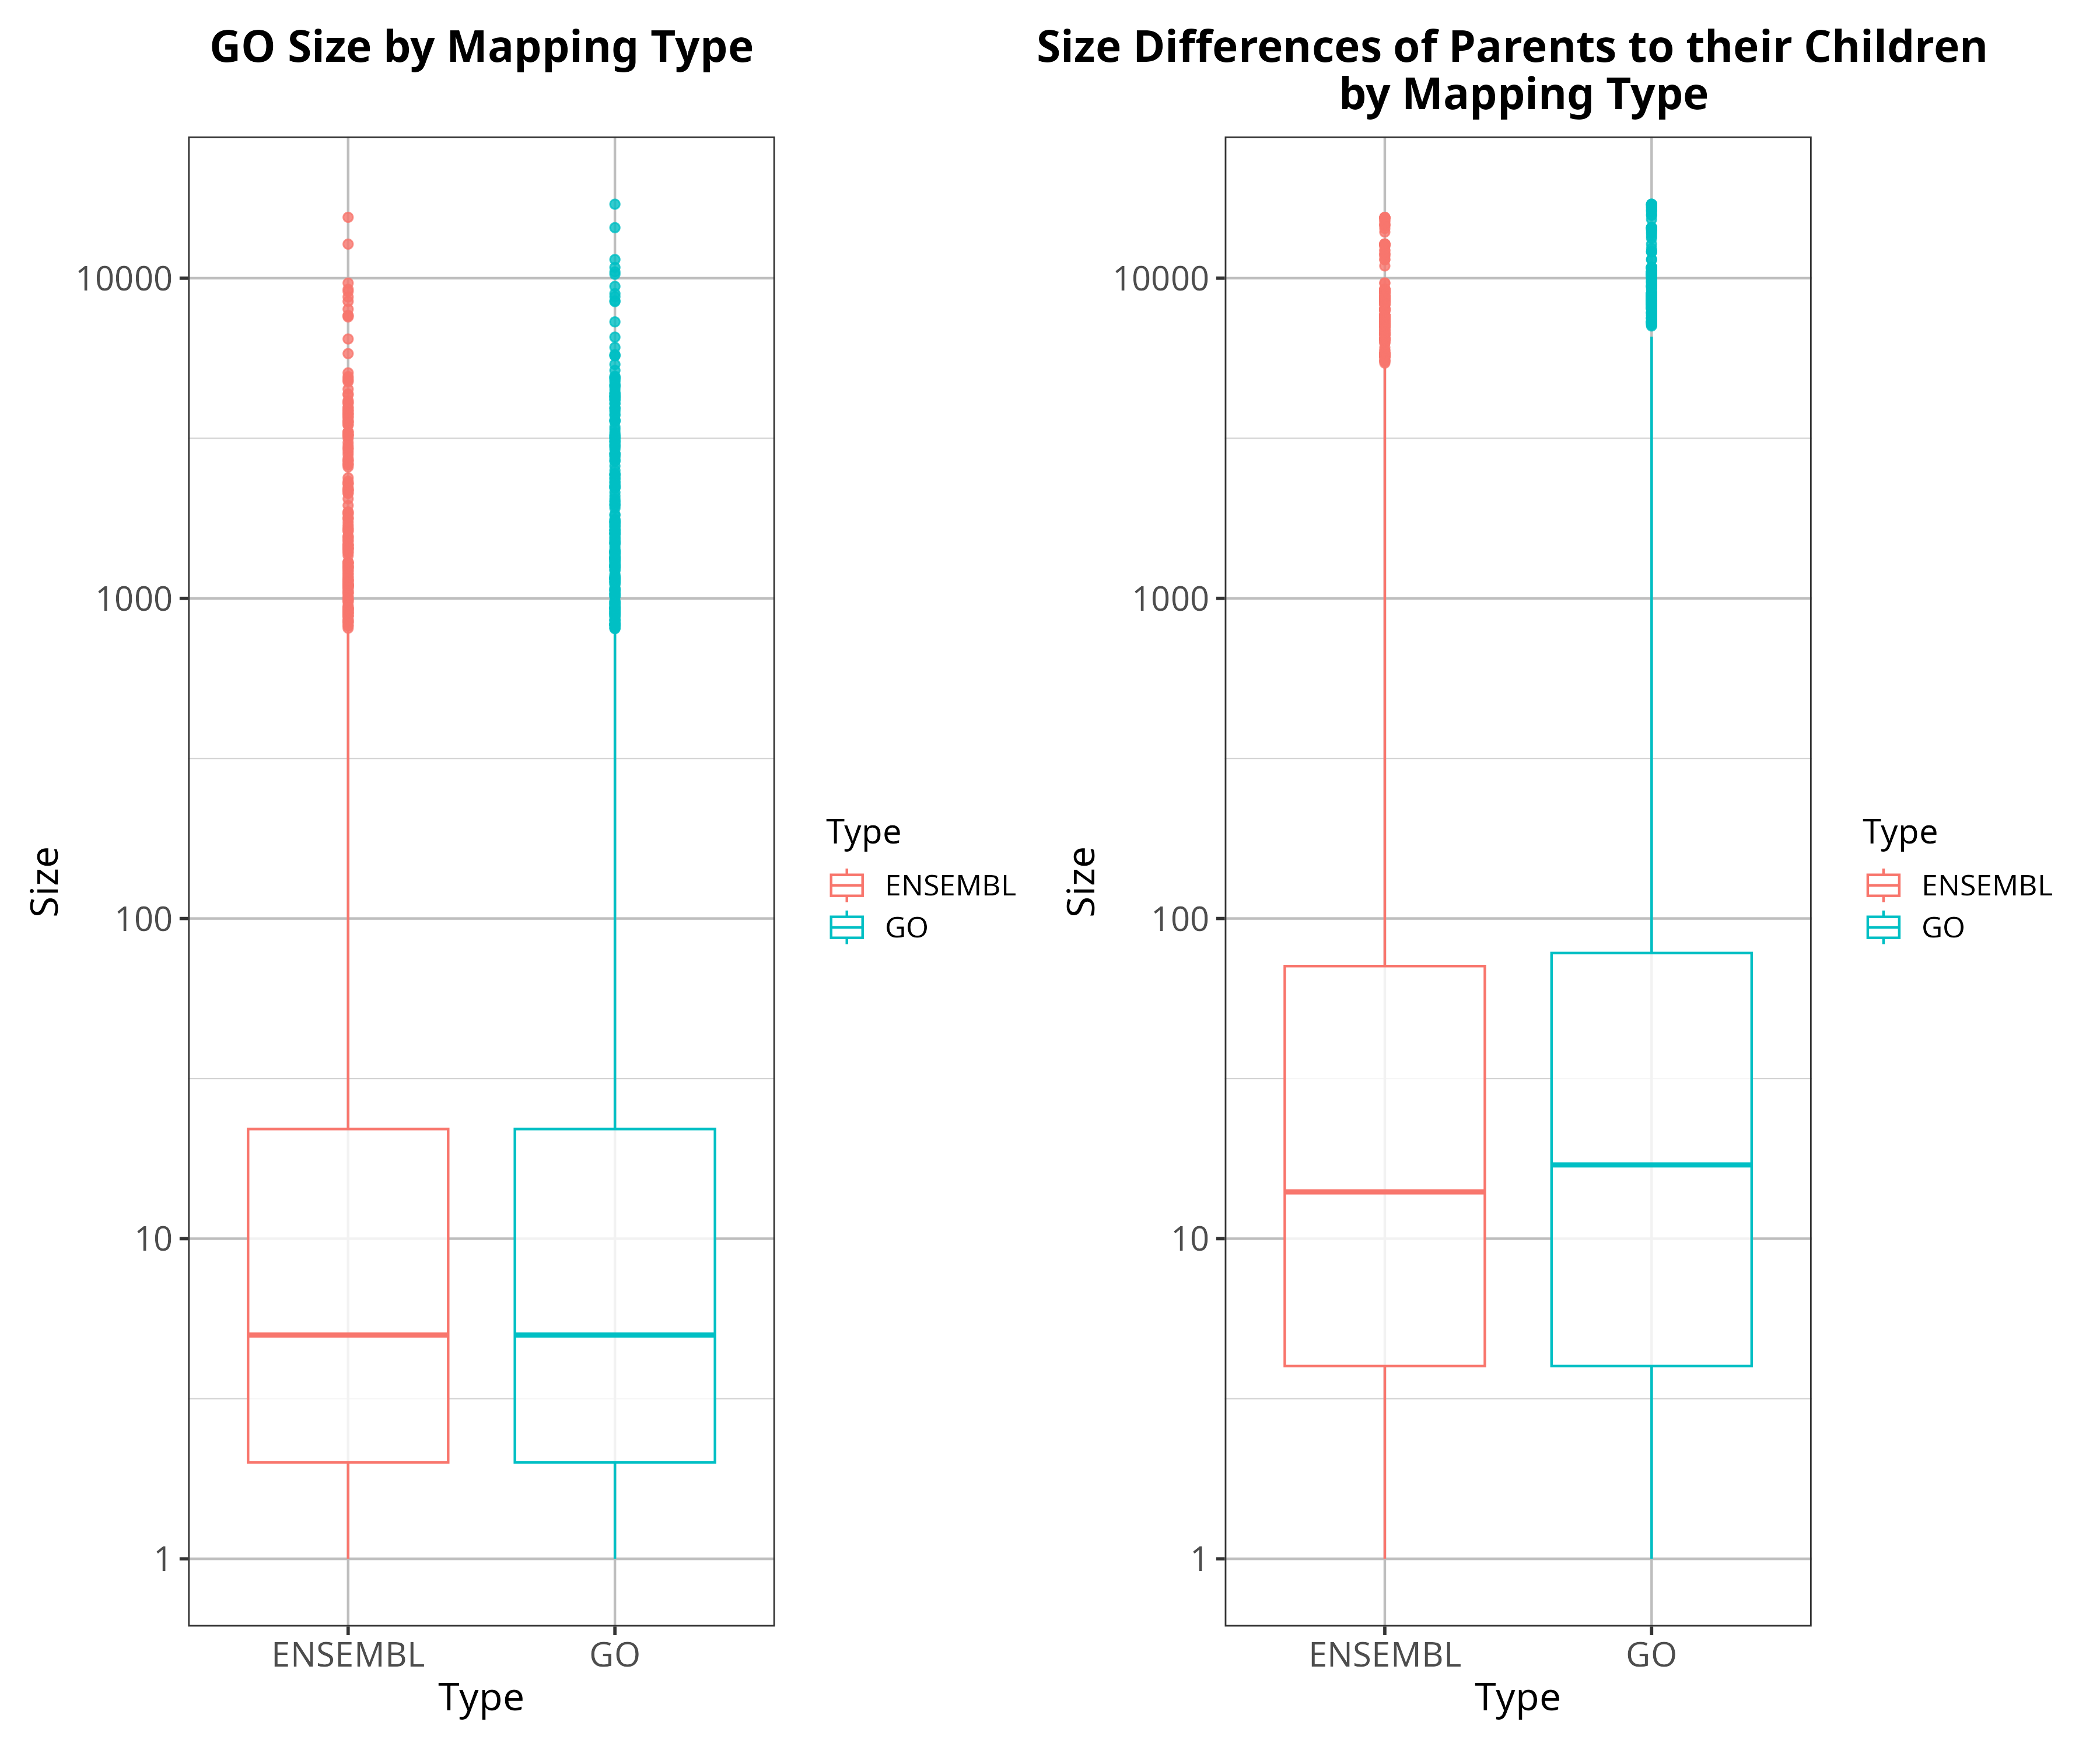
\includegraphics[width=0.8\textwidth]{./plots/goSizes.png}
    \caption{Comparison of gene set sizes in the DAG as well as the difference in gene set sizes between parent and child nodes, per mapping type.}
    \label{fig:-plots-goSizes-png}
\end{figure}

\begin{figure}[htpb]
    \centering
    \begin{minipage}{0.49\textwidth}
        \centering
        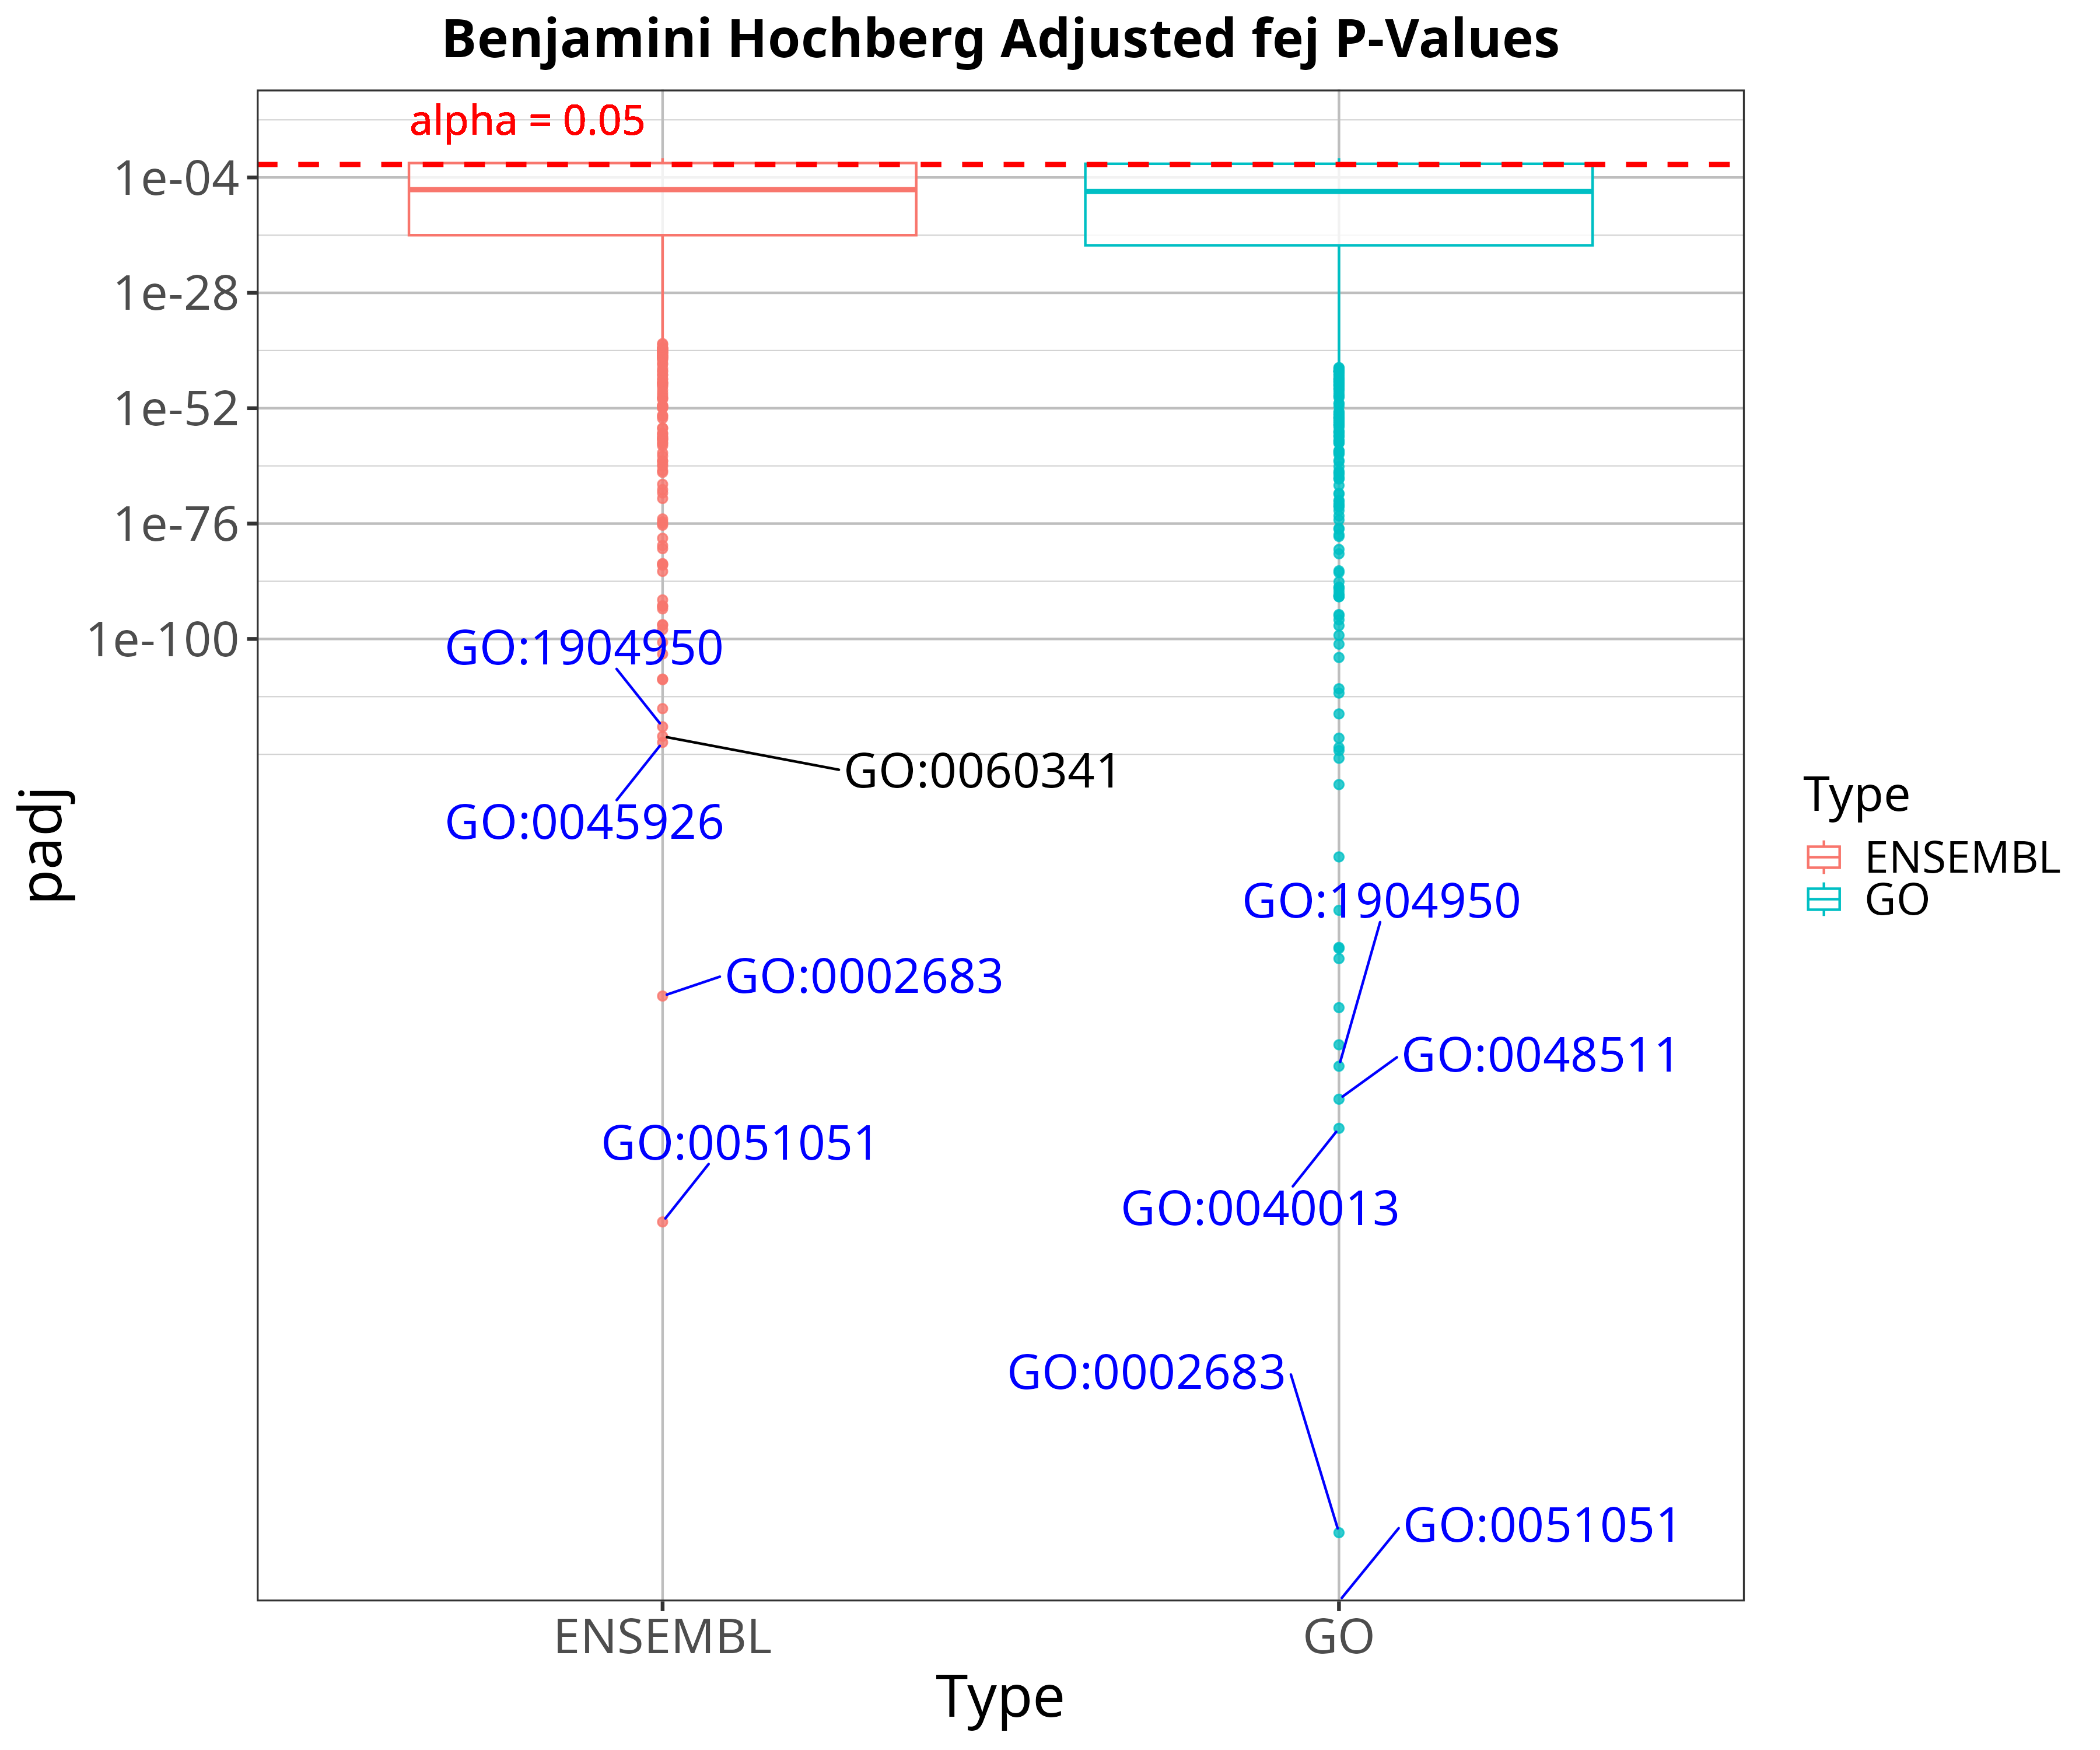
\includegraphics[width=\textwidth]{./plots/BHBoxplotFDRFEJ.png}
        \caption{Boxplot for FDR FEJ}
        \label{fig:boxplot-fdr-fej}
    \end{minipage}
    \hfill
    \begin{minipage}{0.49\textwidth}
        \centering
        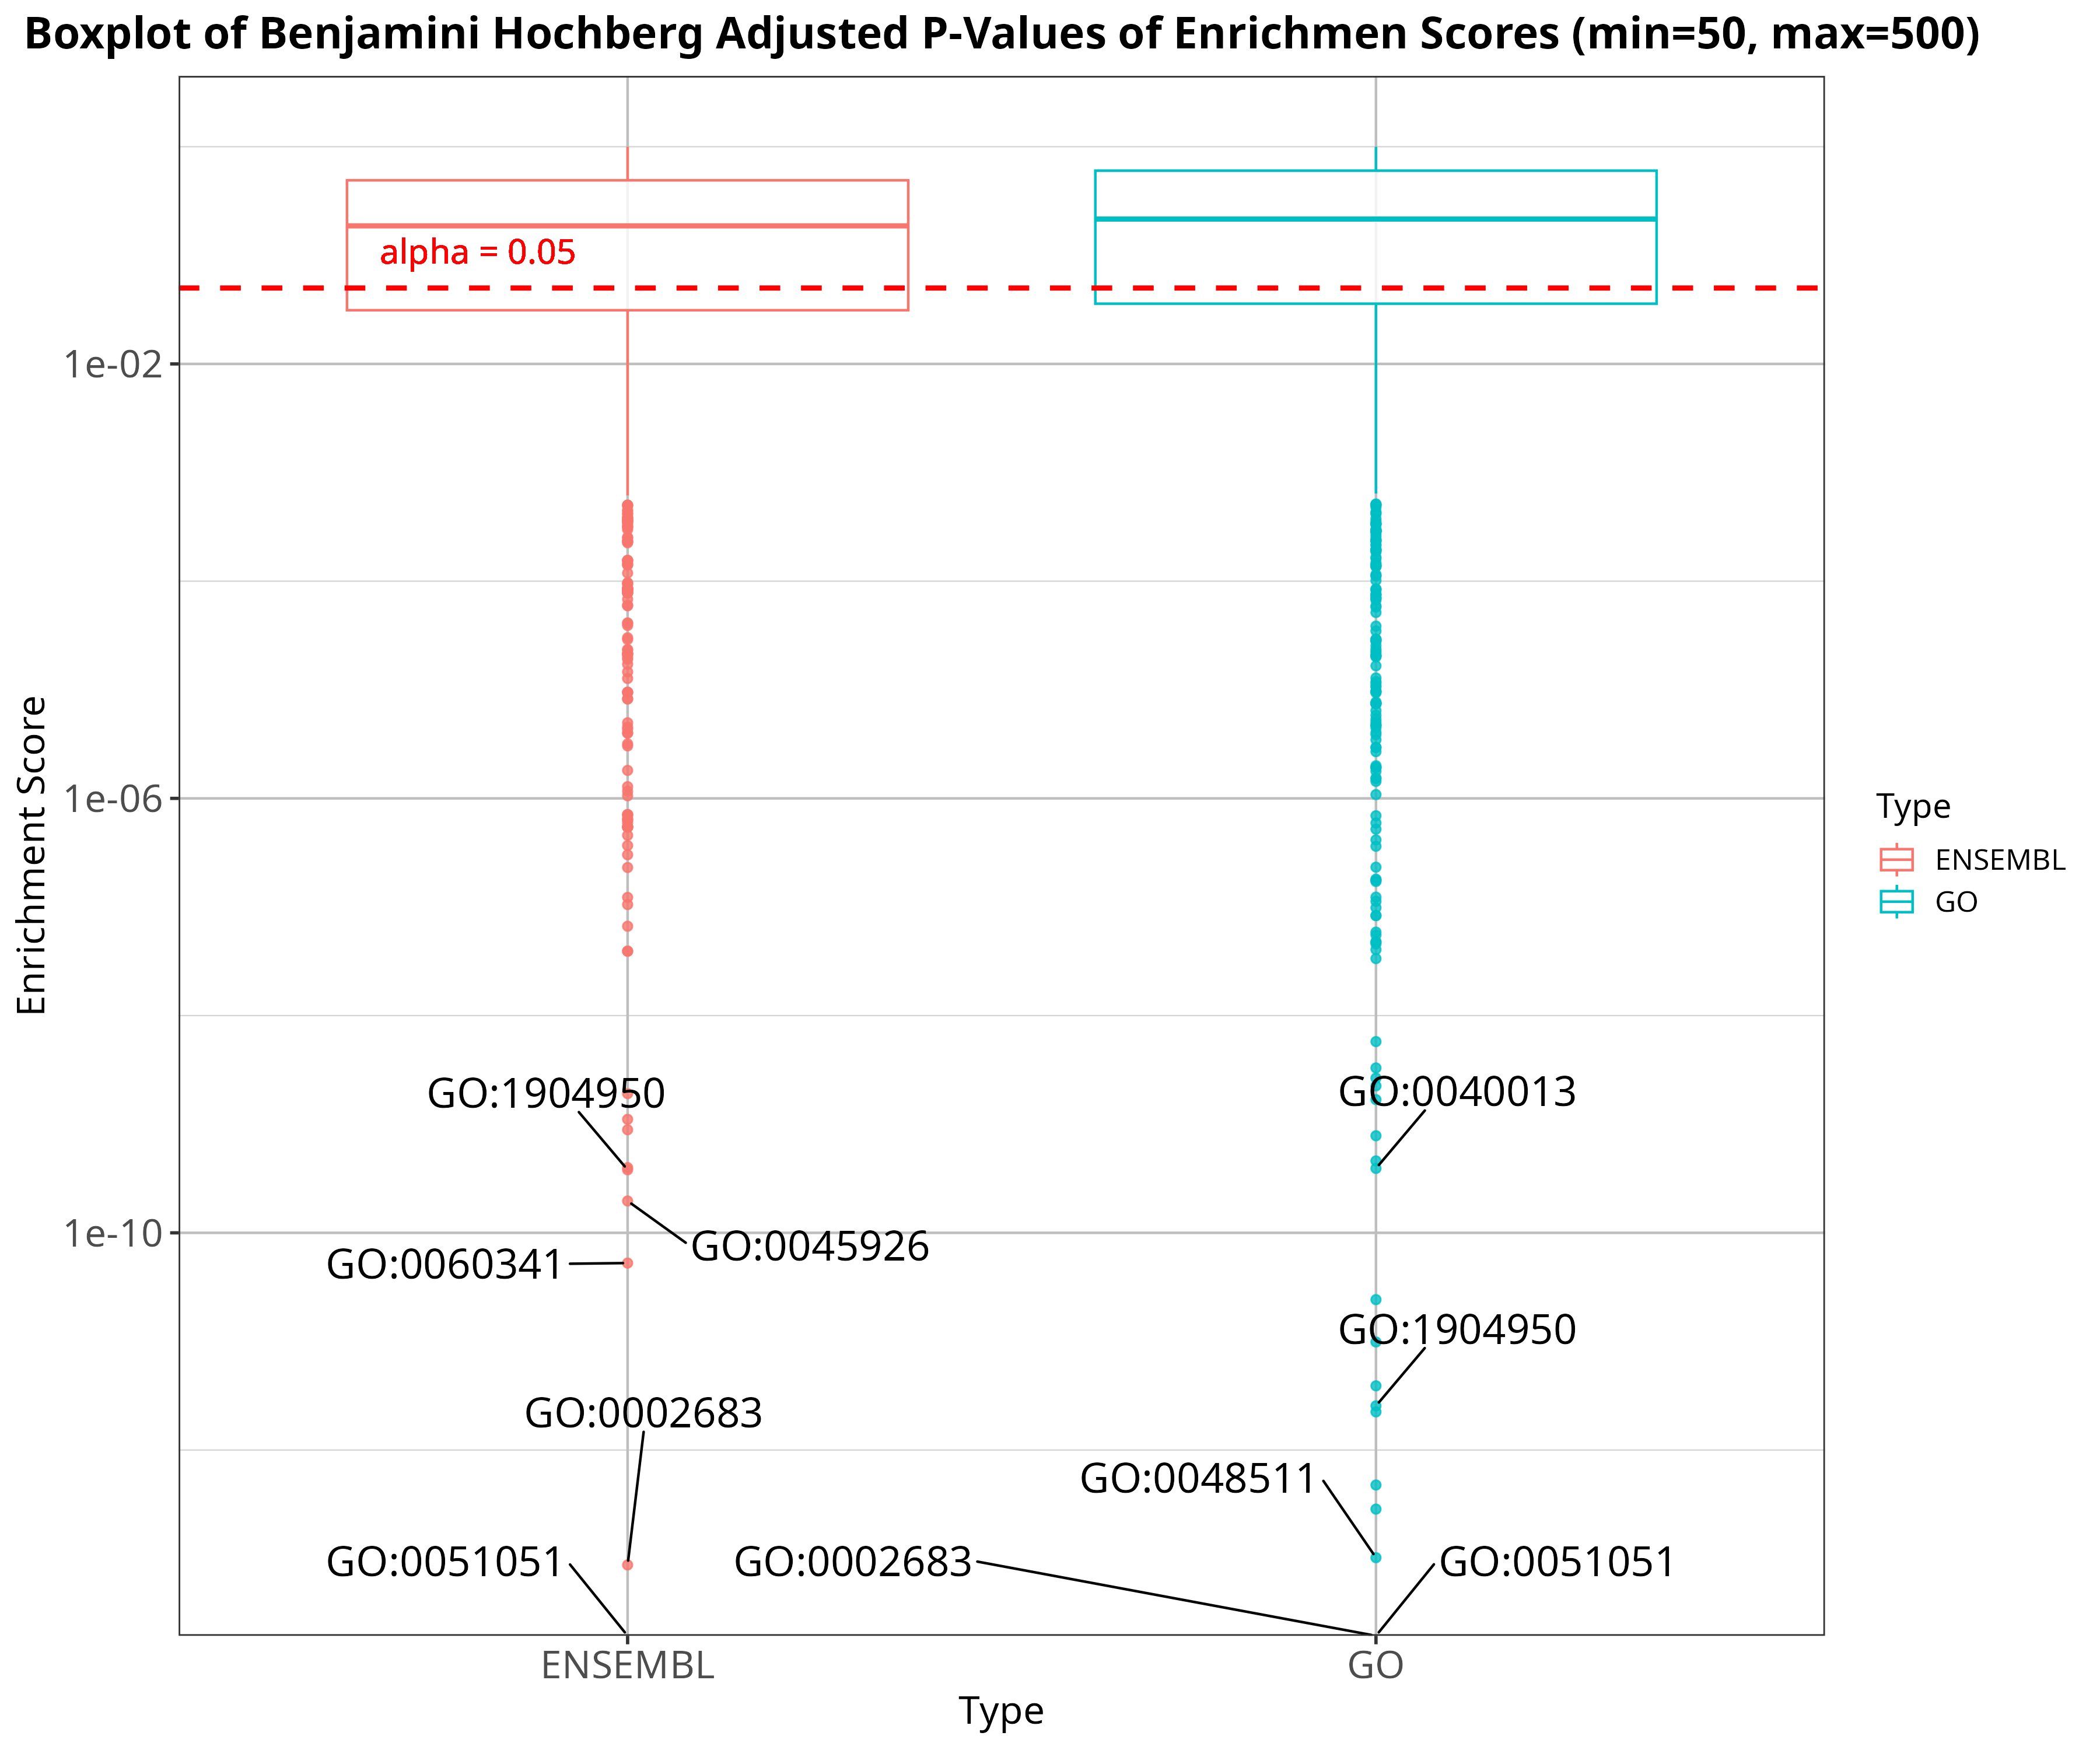
\includegraphics[width=\textwidth]{./plots/BHBoxplotFDRKS.png}
        \caption{Boxplot for FDR KS}
        \label{fig:boxplot-fdr-ks}
    \end{minipage}
\end{figure}

\begin{figure}[htpb]
    \centering
    \begin{minipage}{0.49\textwidth}
        \centering
        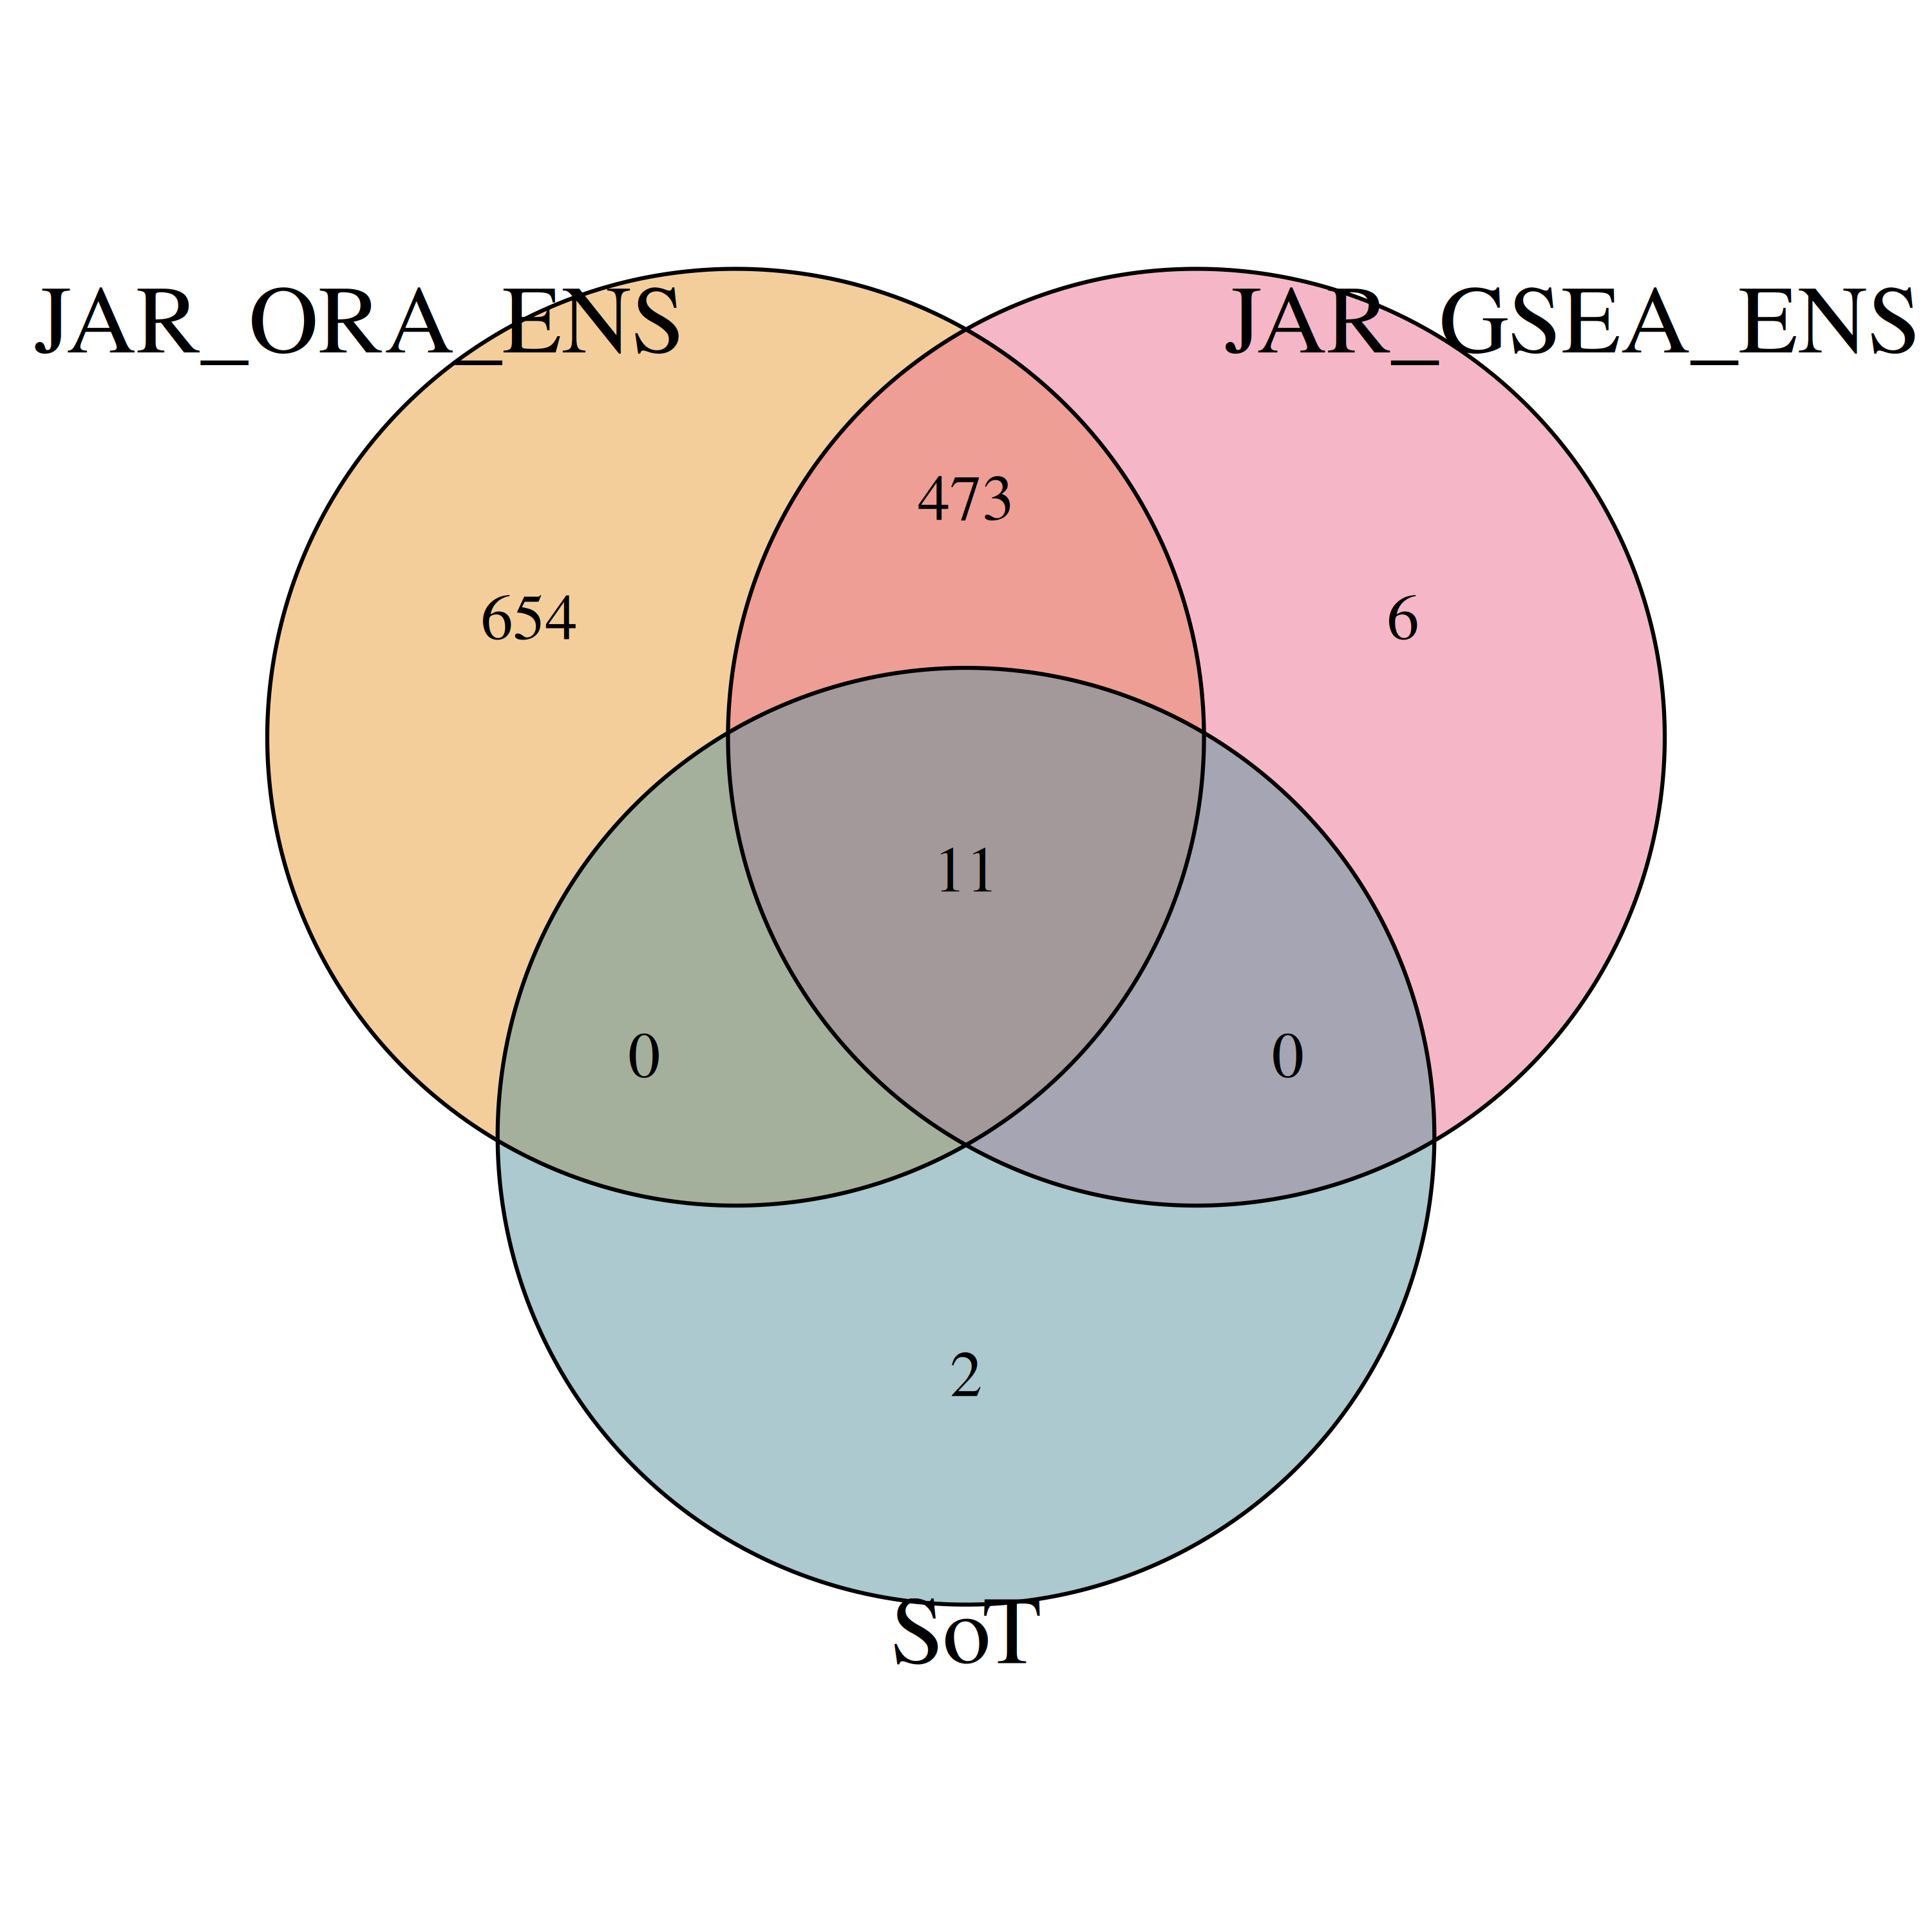
\includegraphics[width=\textwidth]{./plots/ensOverlap.png}
        \caption{Ensembl Overlap Plot, [1] "GO:0098754" "GO:2000242" missing}

        \label{fig:ens-overlap}
    \end{minipage}
    \hfill
    \begin{minipage}{0.49\textwidth}
        \centering
        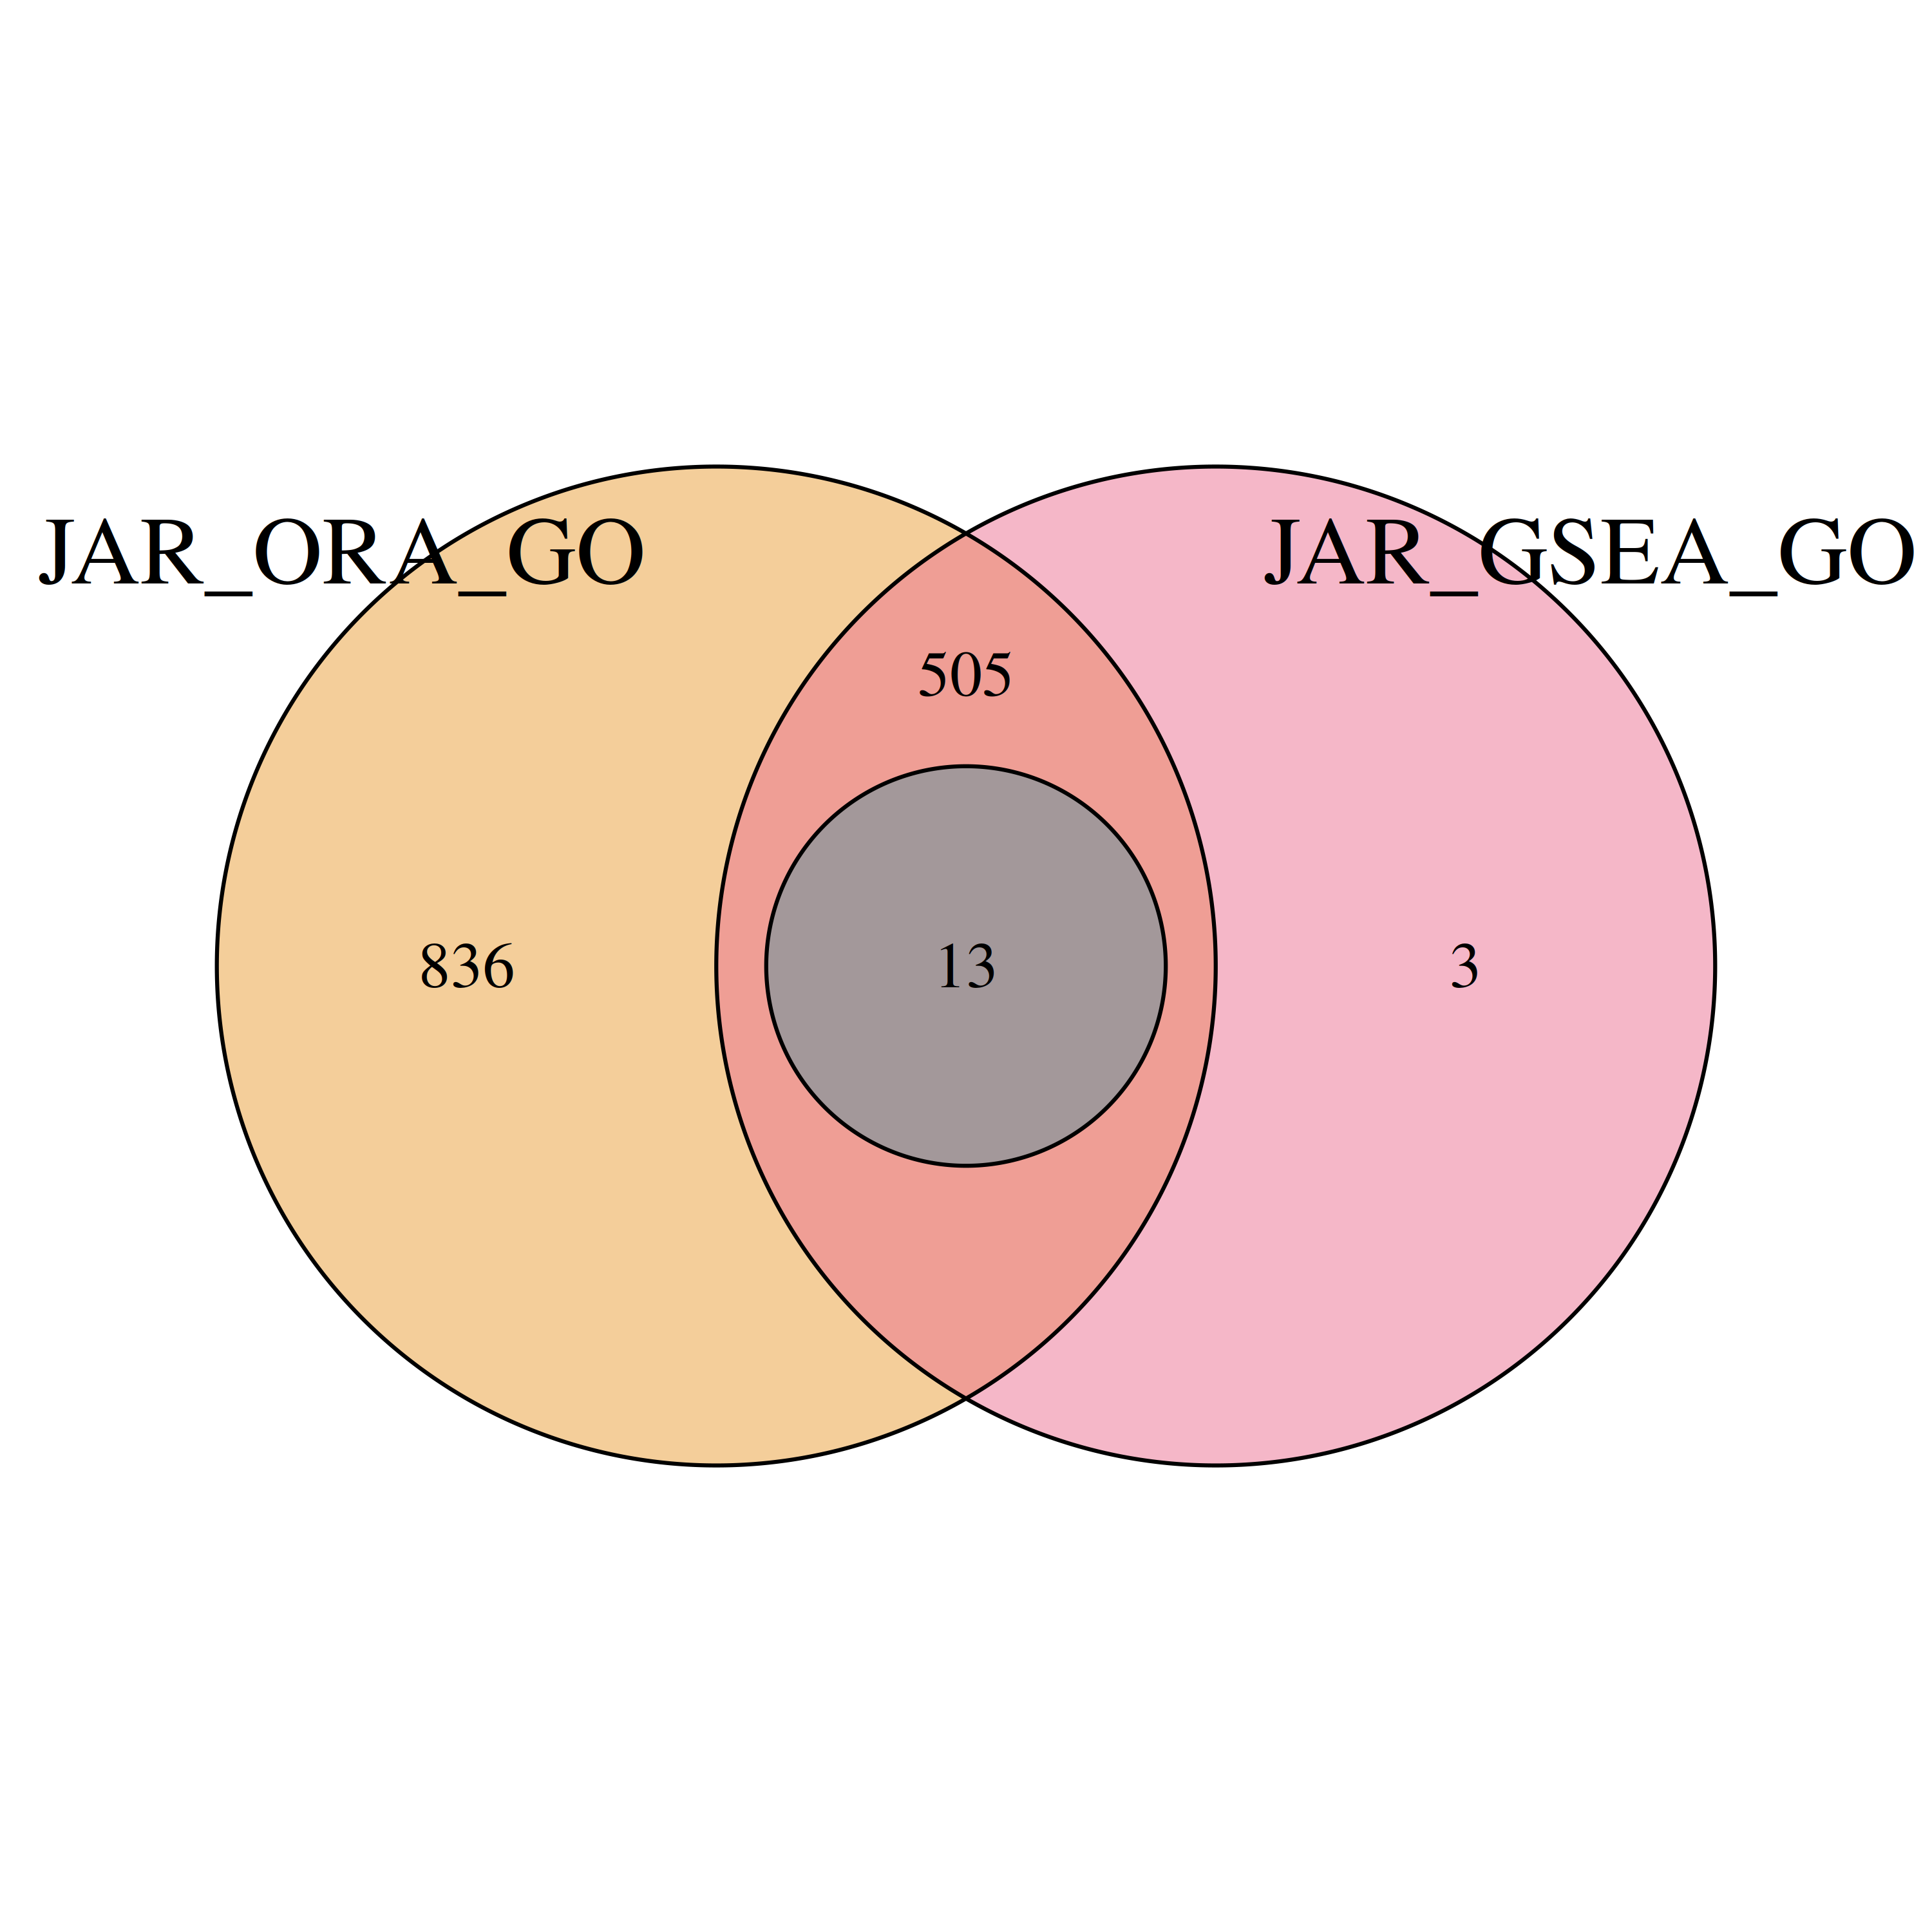
\includegraphics[width=\textwidth]{./plots/goOverlap.png}
        \caption{GO Overlap Plot}
        \label{fig:go-overlap}
    \end{minipage}
\end{figure}

\begin{figure}[htpb]
    \centering
    \begin{minipage}{0.49\textwidth}
        \centering
        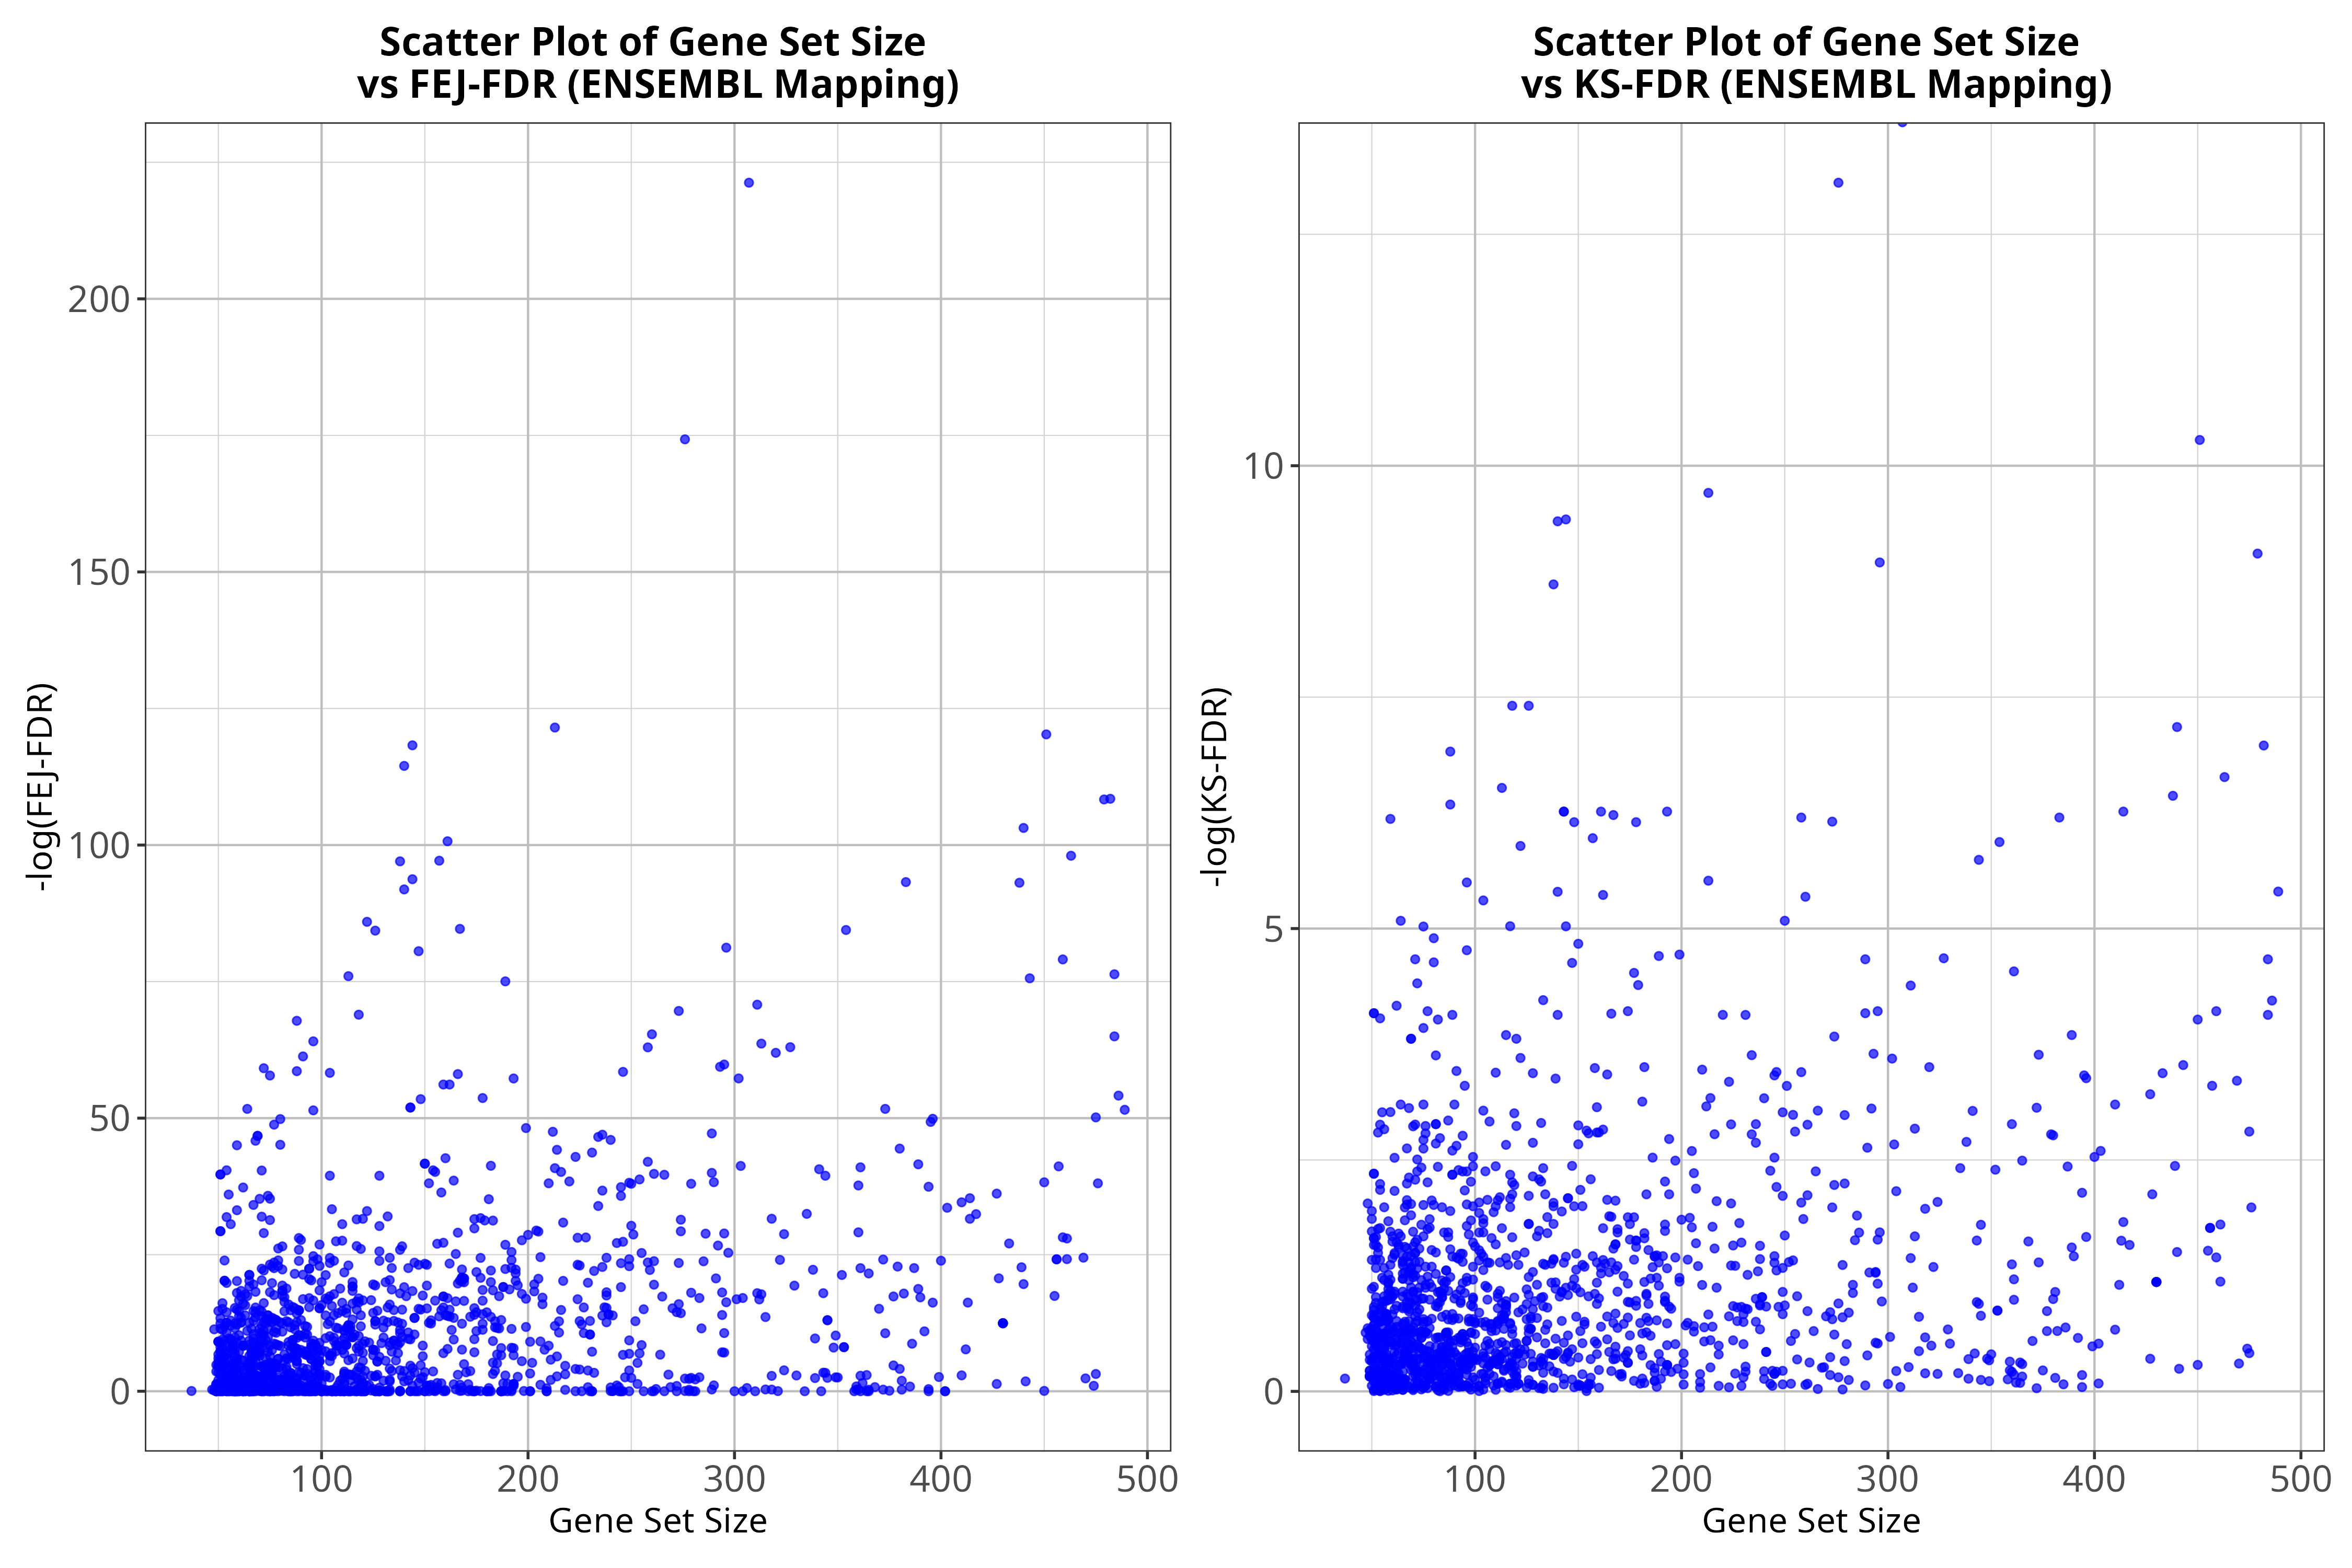
\includegraphics[width=\textwidth]{./plots/ensScatt.png}
        \caption{Ensembl Scatter Plot}
        \label{fig:ens-scatt}
    \end{minipage}
    \hfill
    \begin{minipage}{0.49\textwidth}
        \centering
        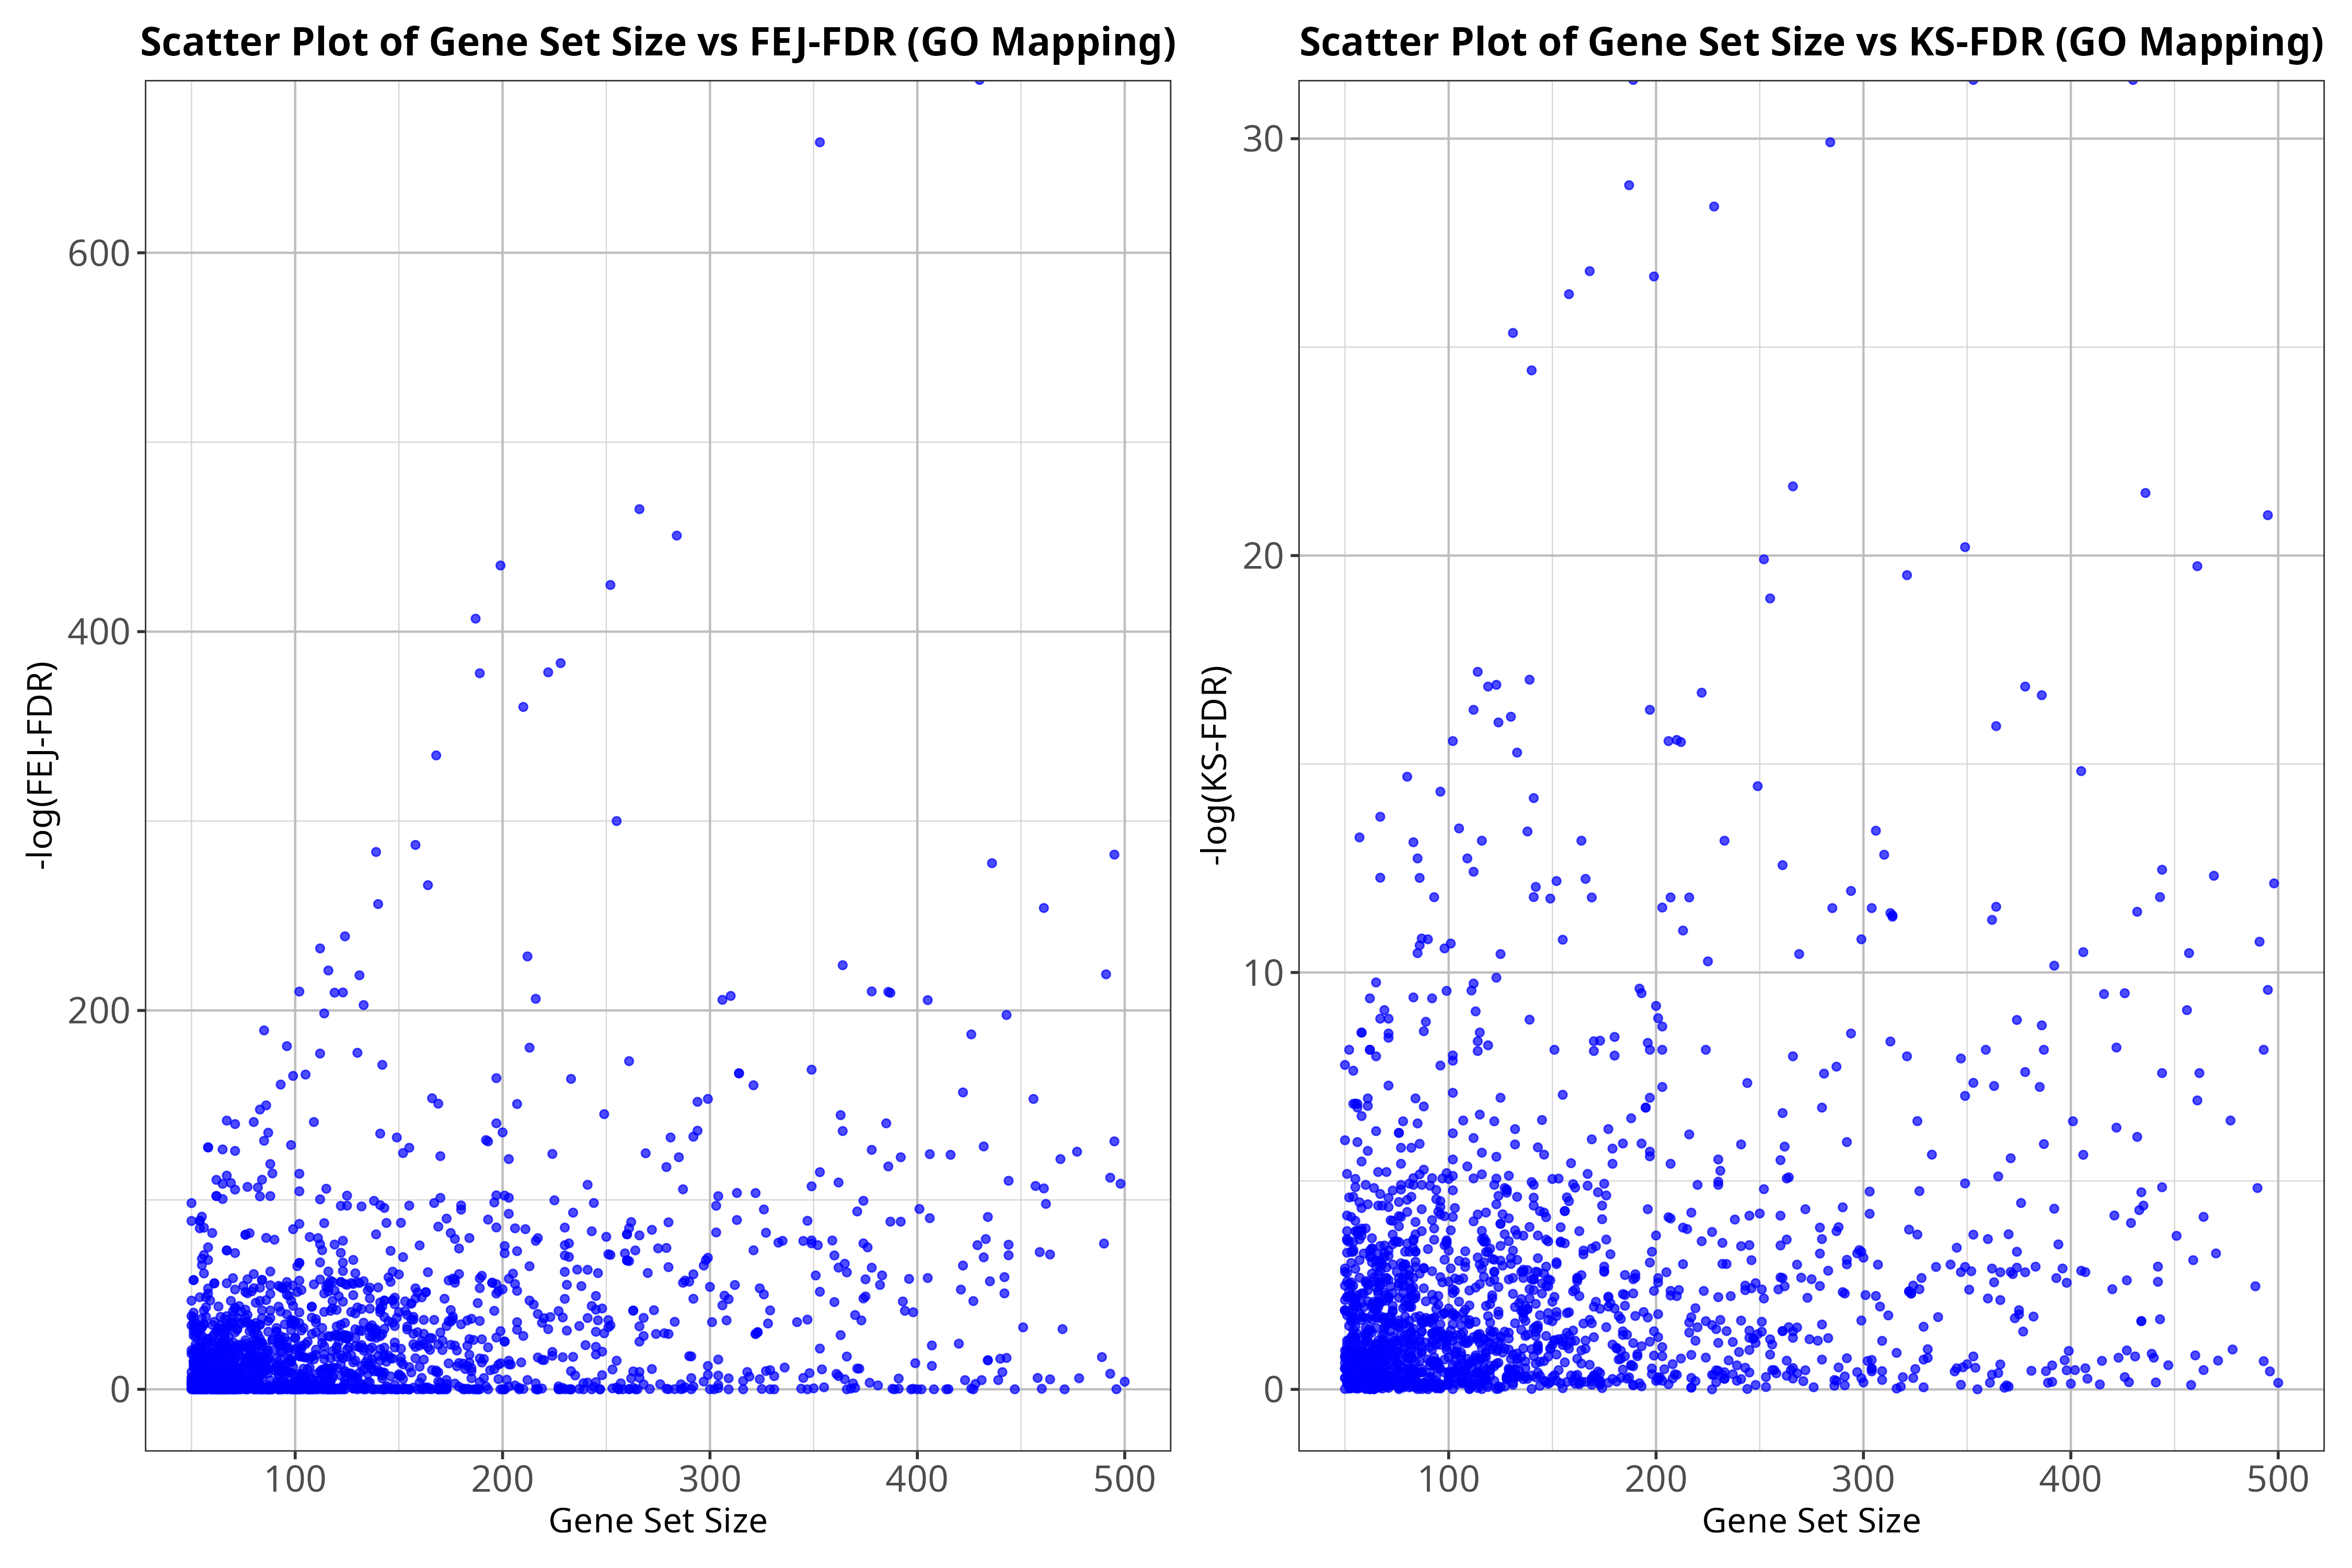
\includegraphics[width=\textwidth]{./plots/goScatt.png}
        \caption{GO Scatter Plot}
        \label{fig:go-scatt}
    \end{minipage}
\end{figure}

\subsection{Comparison with Online Tool gProfiler (ORA)}\label{sec:Comparison-of-ORA}
\begin{figure}[htpb]
    \centering
    \begin{minipage}{0.49\textwidth}
        \centering
        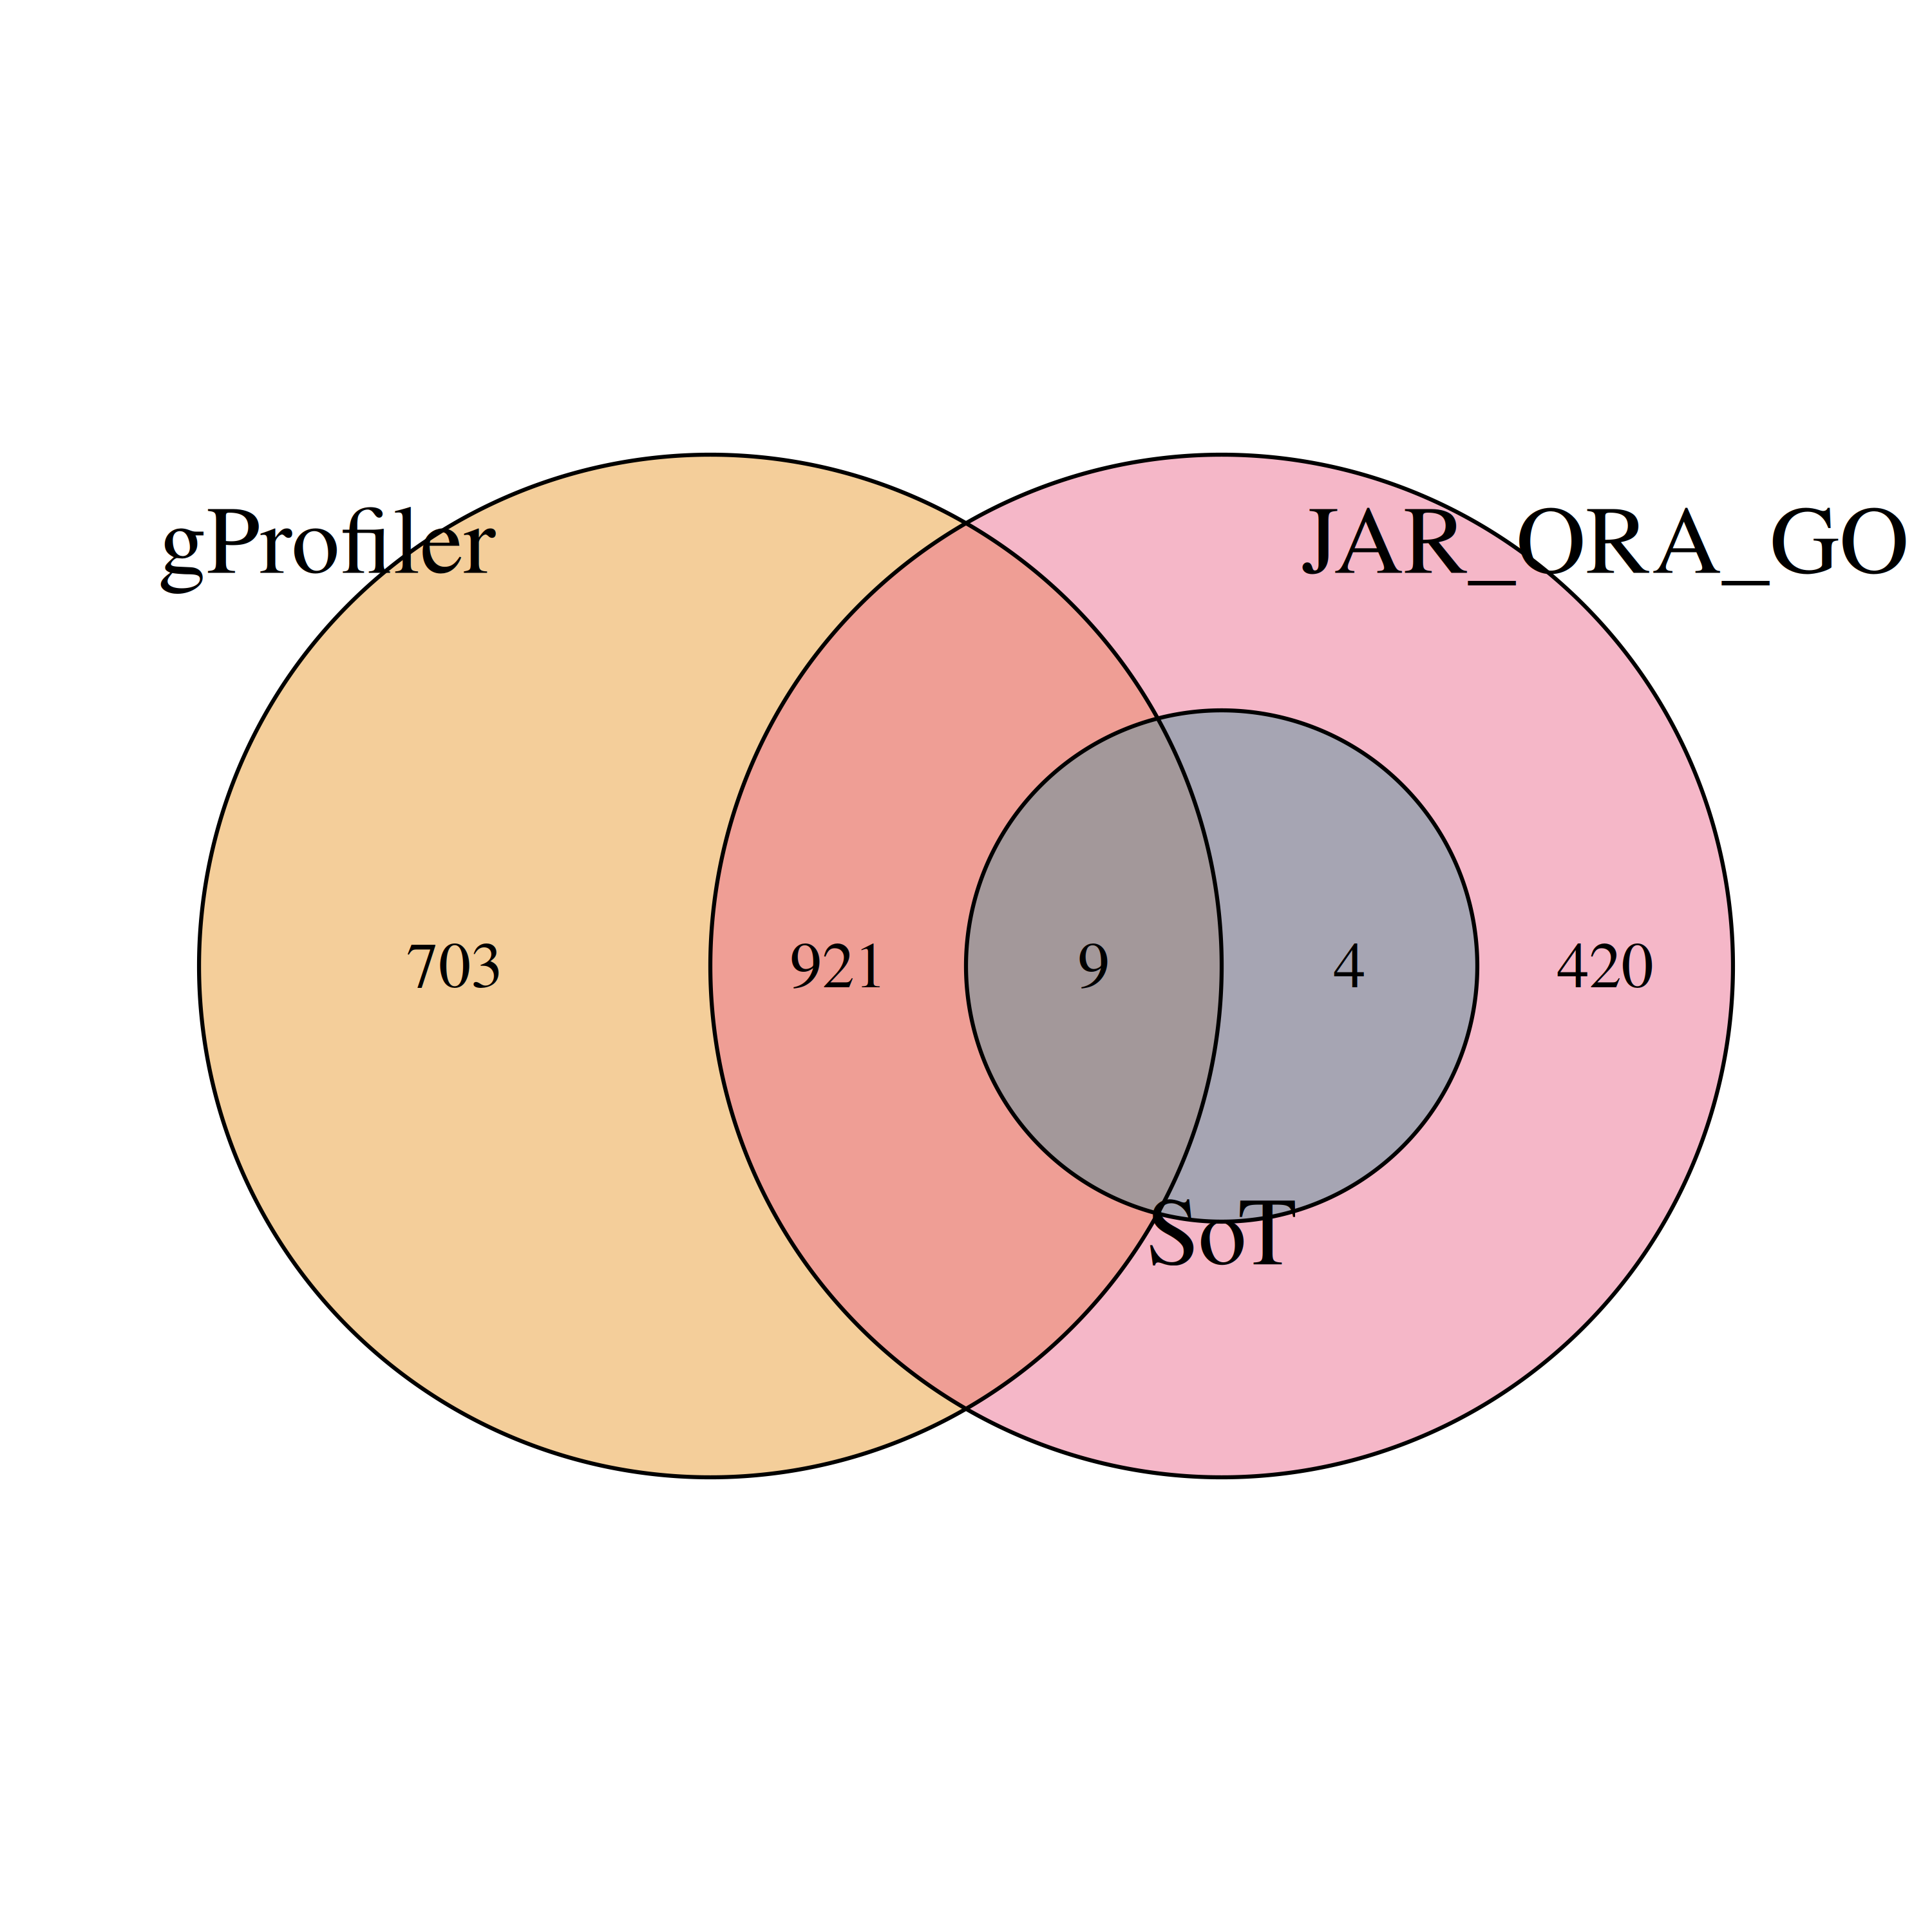
\includegraphics[width=\textwidth]{./plots/go_mappingCompgProfiler.png}
        \caption{GO Mapping Comparison - gProfiler}
        \label{fig:go-mapping-gprofiler}
    \end{minipage}
    \hfill
    \begin{minipage}{0.49\textwidth}
        \centering
        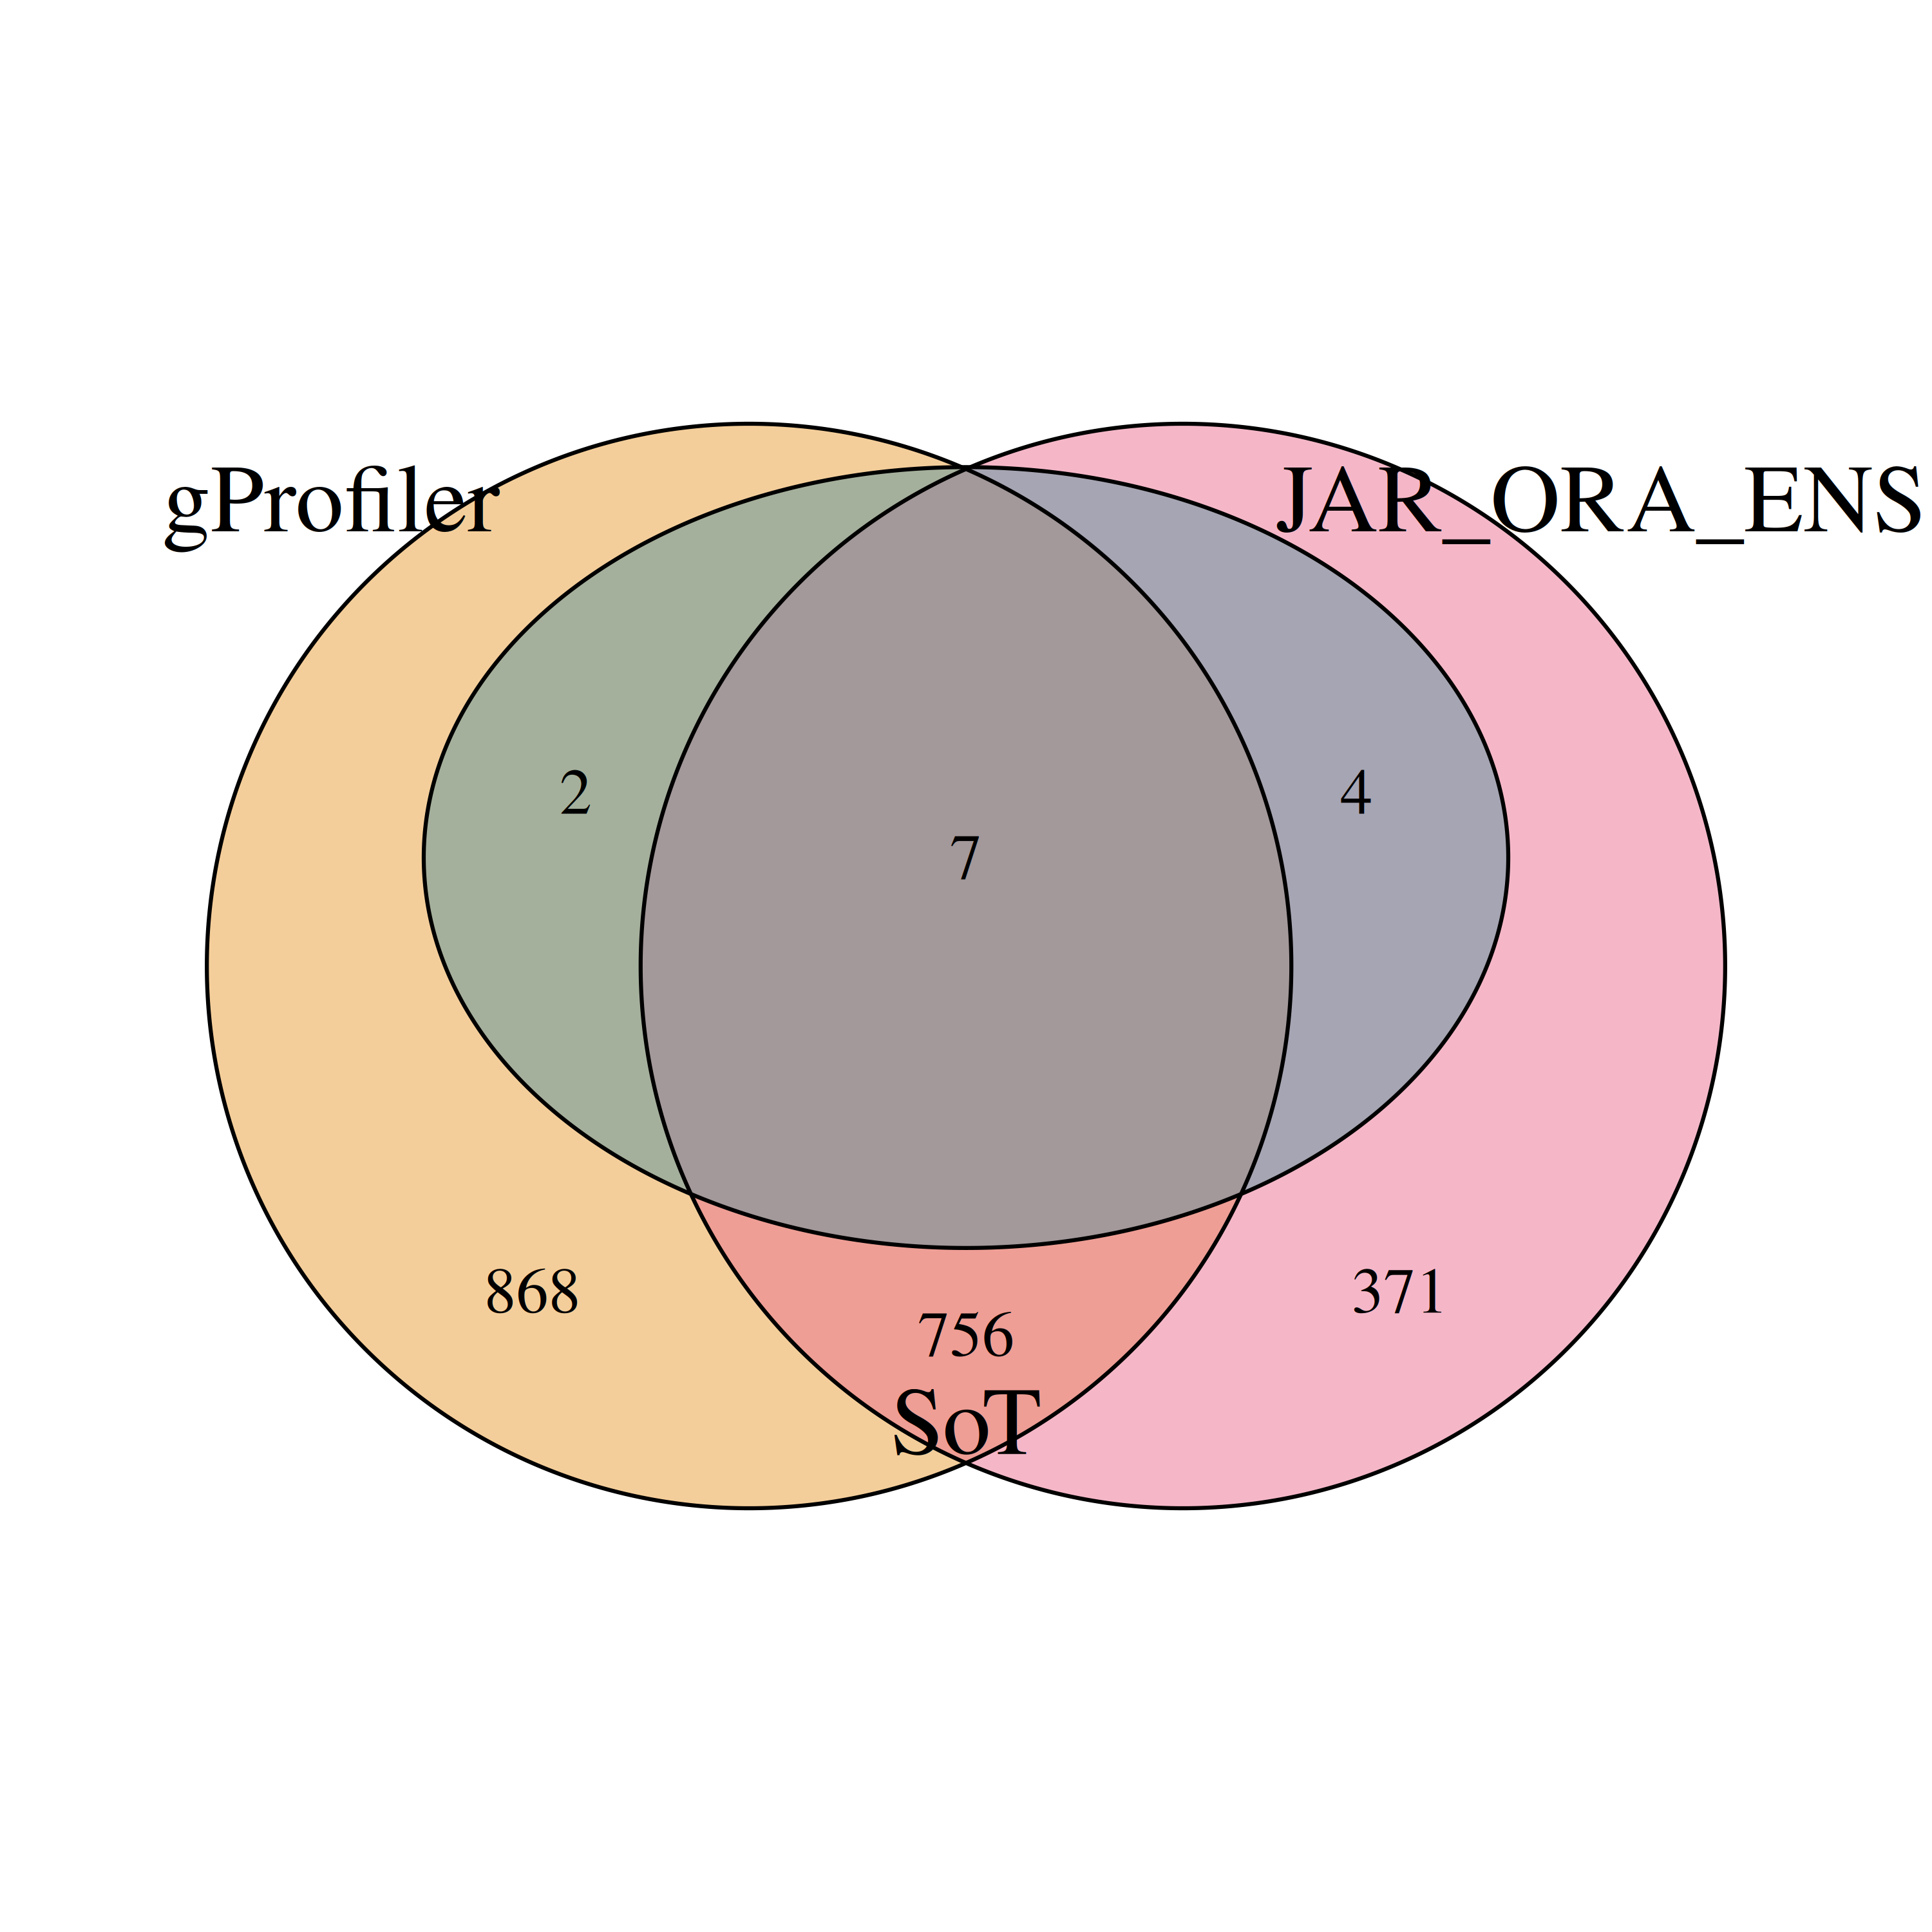
\includegraphics[width=\textwidth]{./plots/ens_mappingCompgProfiler.png}
        \caption{Ensembl Mapping Comparison - gProfiler $\to$ "GO:2000242" "GO:0098754" not found by our JAR} 

        \label{fig:ens-mapping-gprofiler}
    \end{minipage}
\end{figure}
\subsection{Comparison with R library fgsea (GSEA)}\label{sec:Comparison-of-GSEA}
\begin{figure}[htpb]
    \centering
    \begin{minipage}{0.49\textwidth}
        \centering
        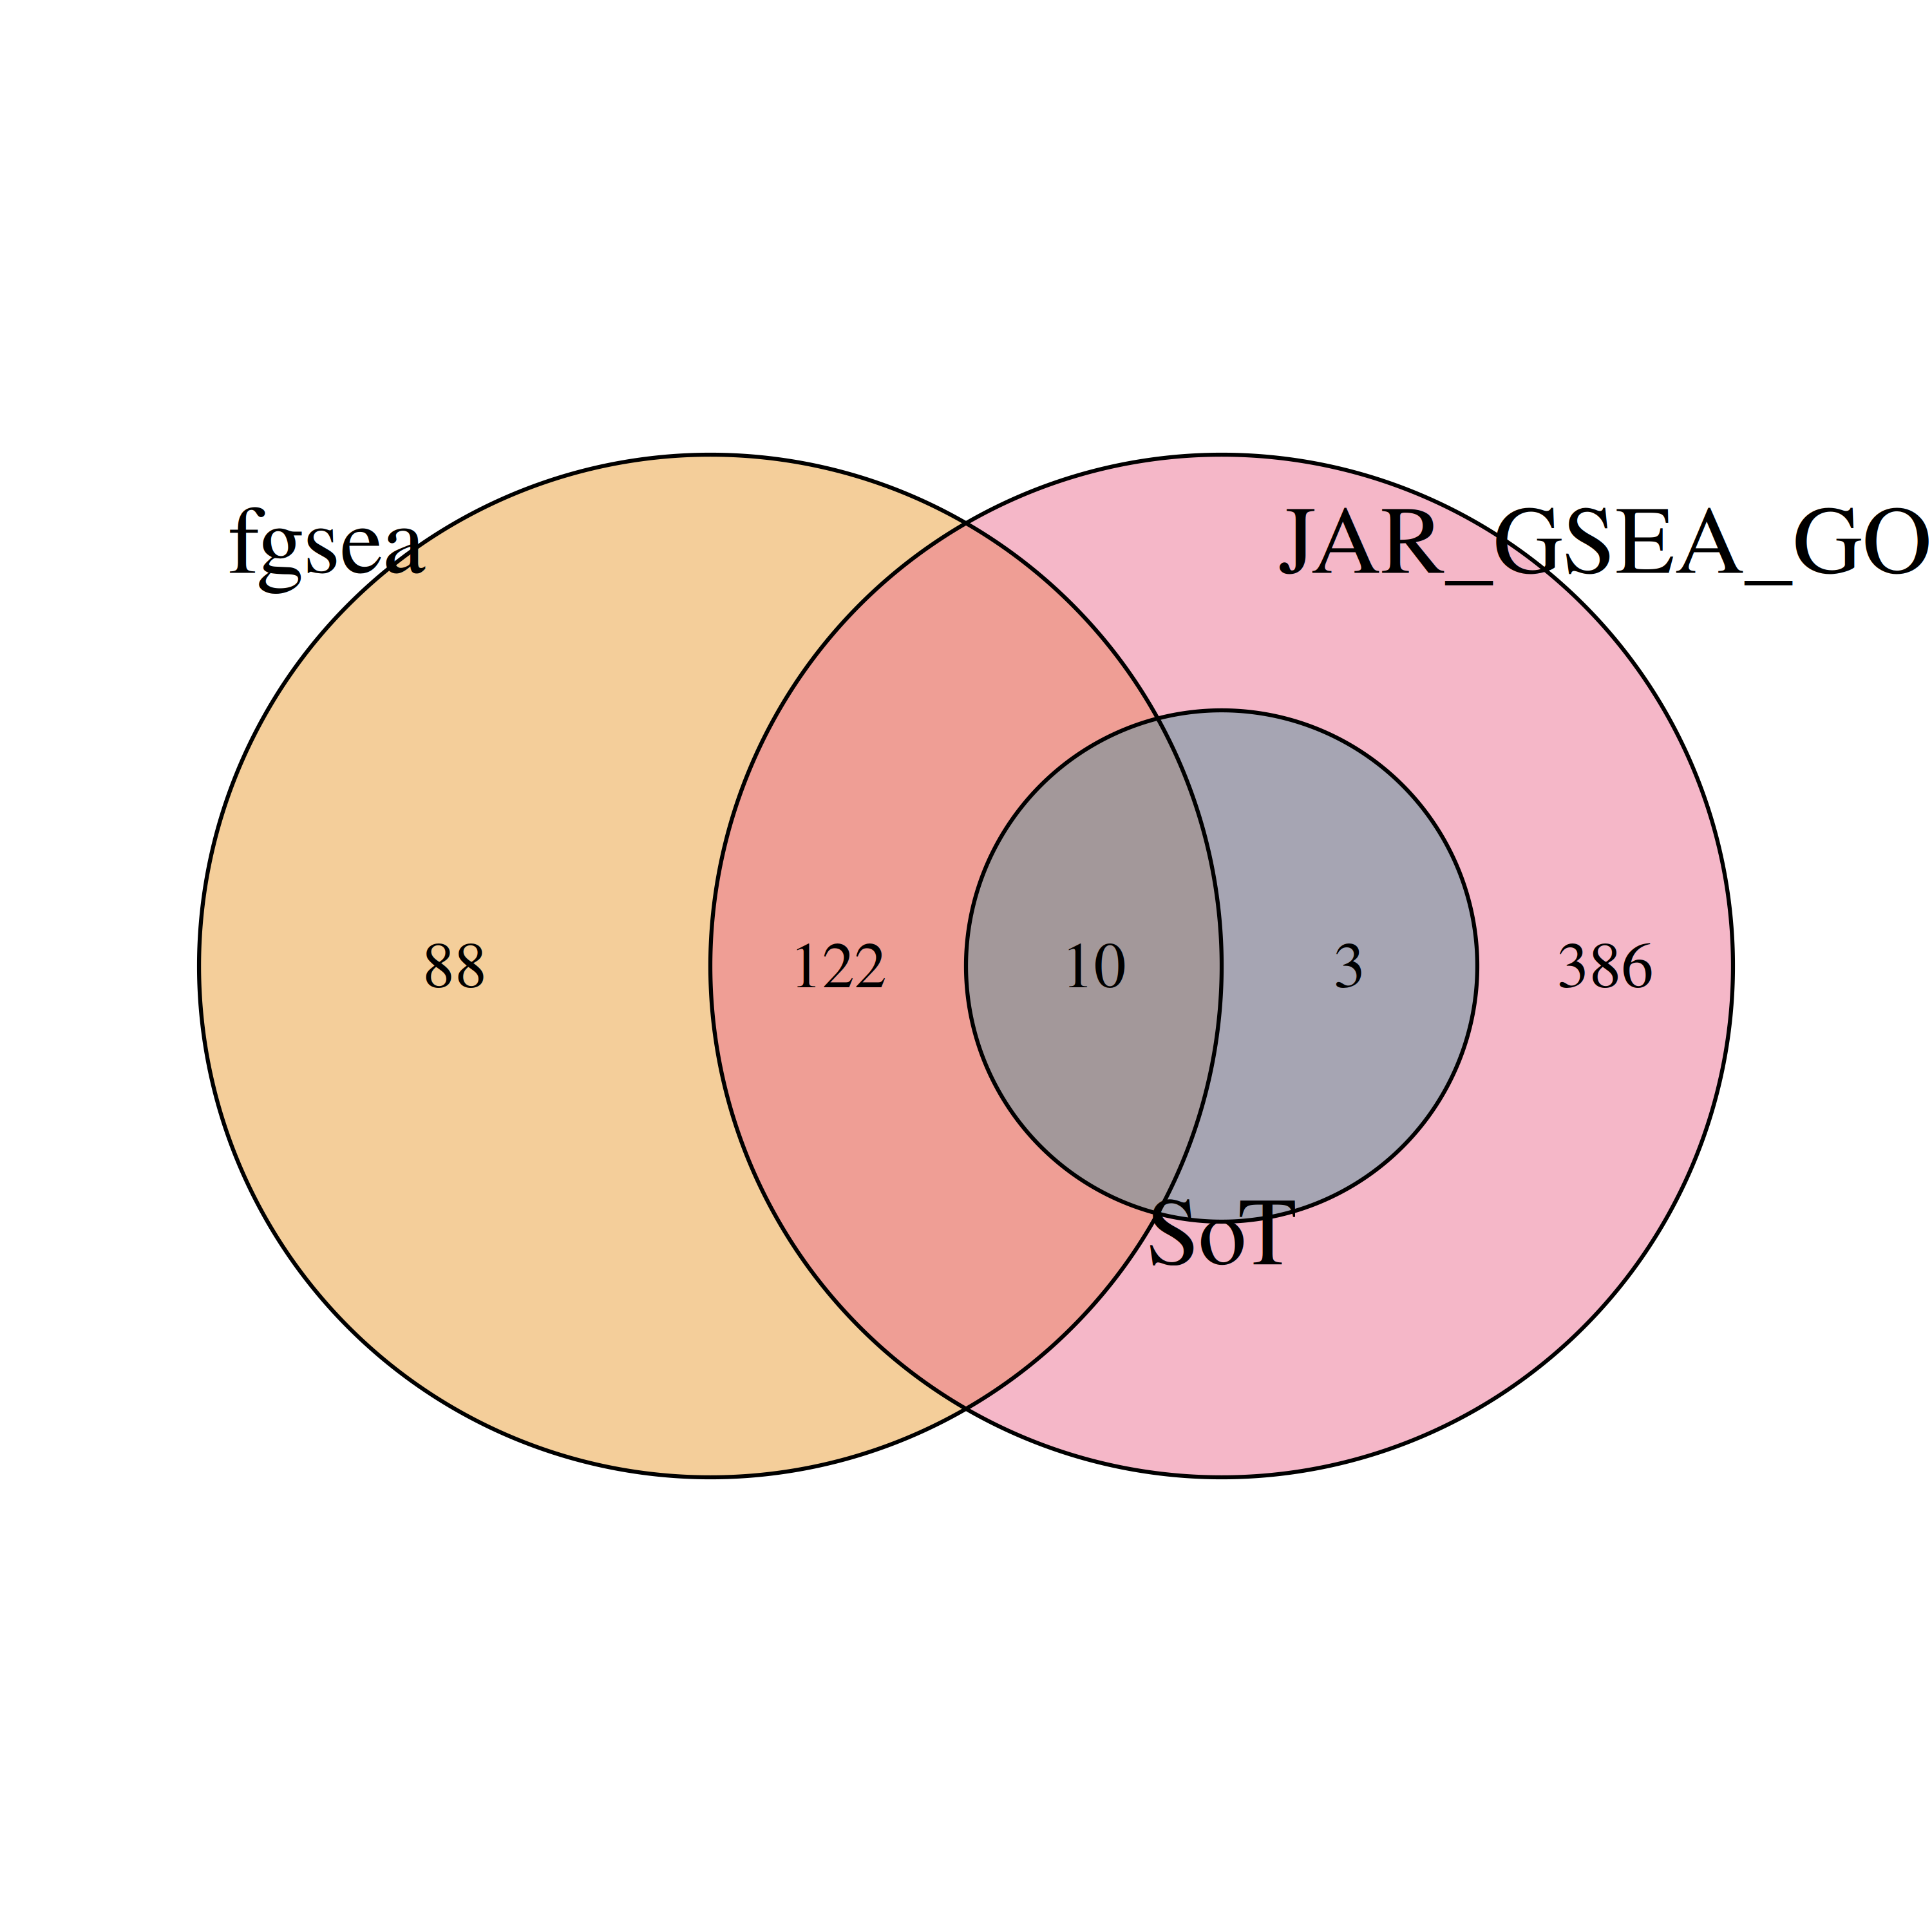
\includegraphics[width=\textwidth]{./plots/go_mappingCompfgsea.png}
        \caption{GO Mapping Comparison - fgsea}
        \label{fig:go-mapping-fgsea}
    \end{minipage}
    \hfill
    \begin{minipage}{0.49\textwidth}
        \centering
        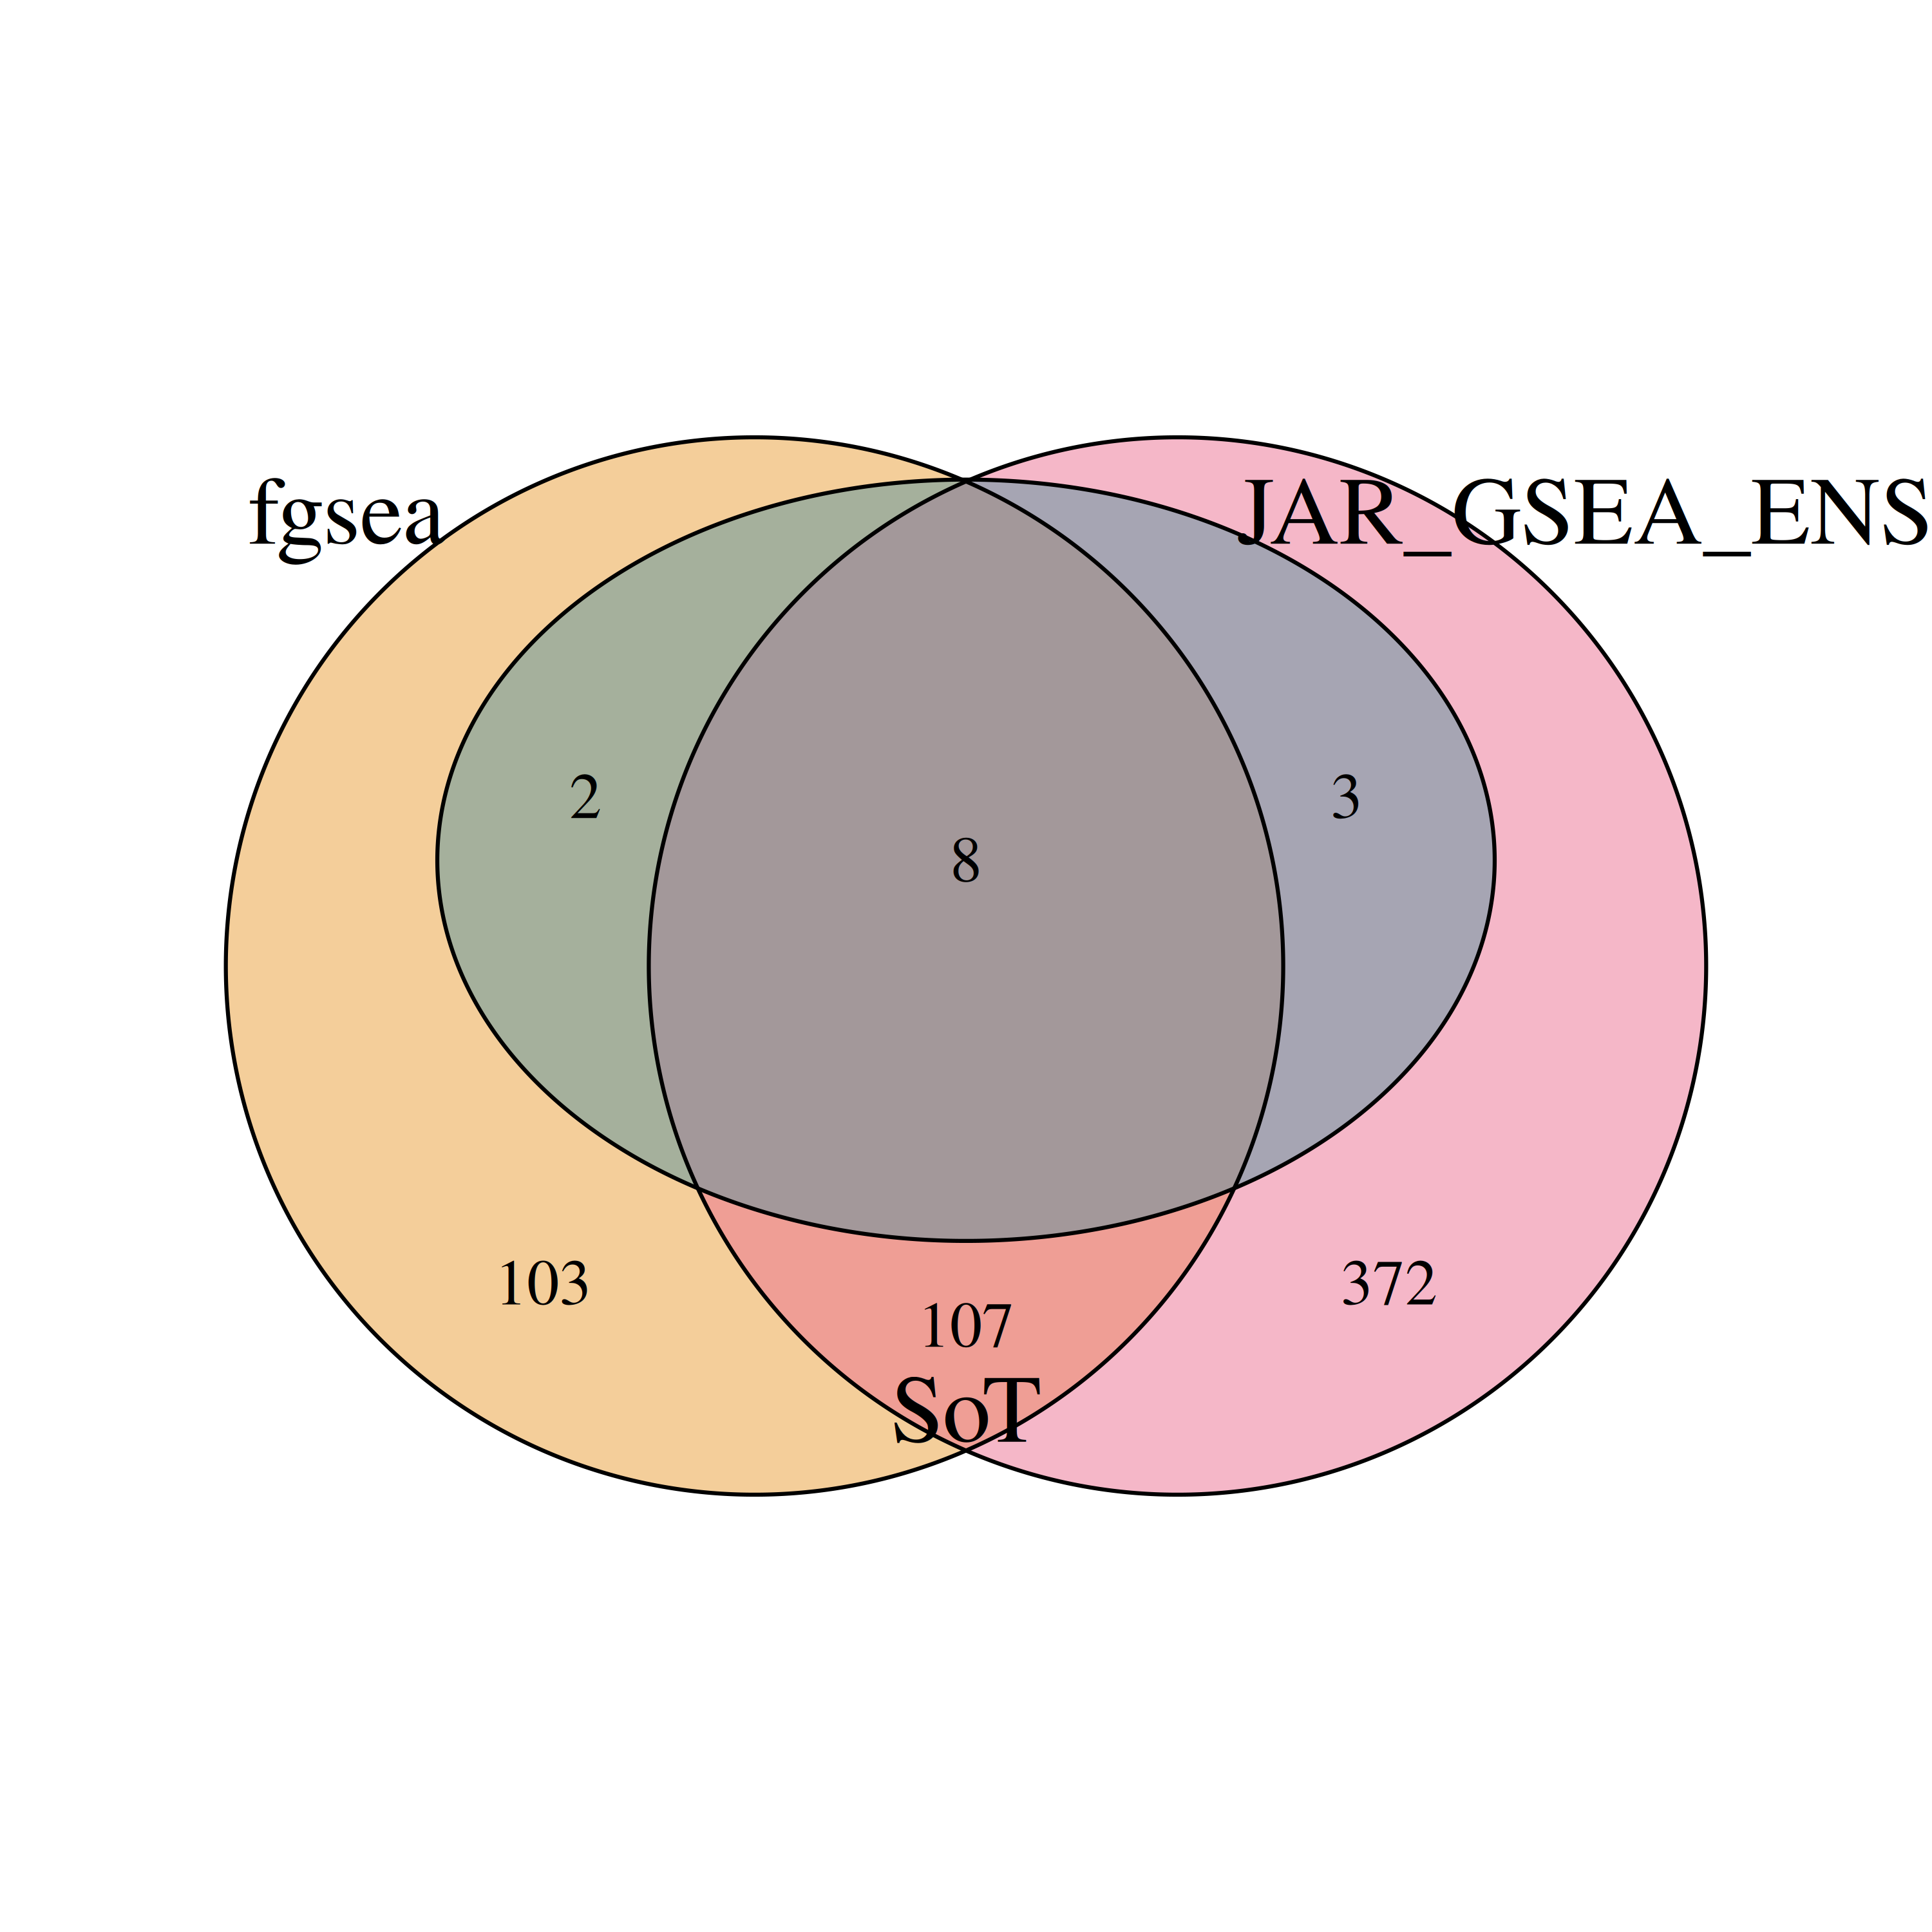
\includegraphics[width=\textwidth]{./plots/ens_mappingCompgfgsea.png}
        \caption{Ensembl Mapping Comparison - fgsea $\to$ "GO:0098754" "GO:2000242" missing}
        \label{fig:ens-mapping-fgsea}
    \end{minipage}
\end{figure}
% ------------------------------------------------------------------------------





% ------------------------------------------------------------------------------
\printbibliography
% ------------------------------------------------------------------------------


\end{document}
